\chapter{Implementarea soluției}

Prin parcurgerea acestui capitol, cititorul va avea o imagine de ansamblu asupra modului în care senzorii sunt integrați în aplicație, cum este realizată comunicarea cu serverul și care sunt aspectele legate de programarea și funcționalitatea aplicației mobile. Aceste informații sunt esențiale pentru a înțelege arhitectura (Figura \ref{fig:arhitectura}) și funcționalitatea aplicației în cadrul sistemului smart home propus.

\begin{figure}[h]
	\centering
	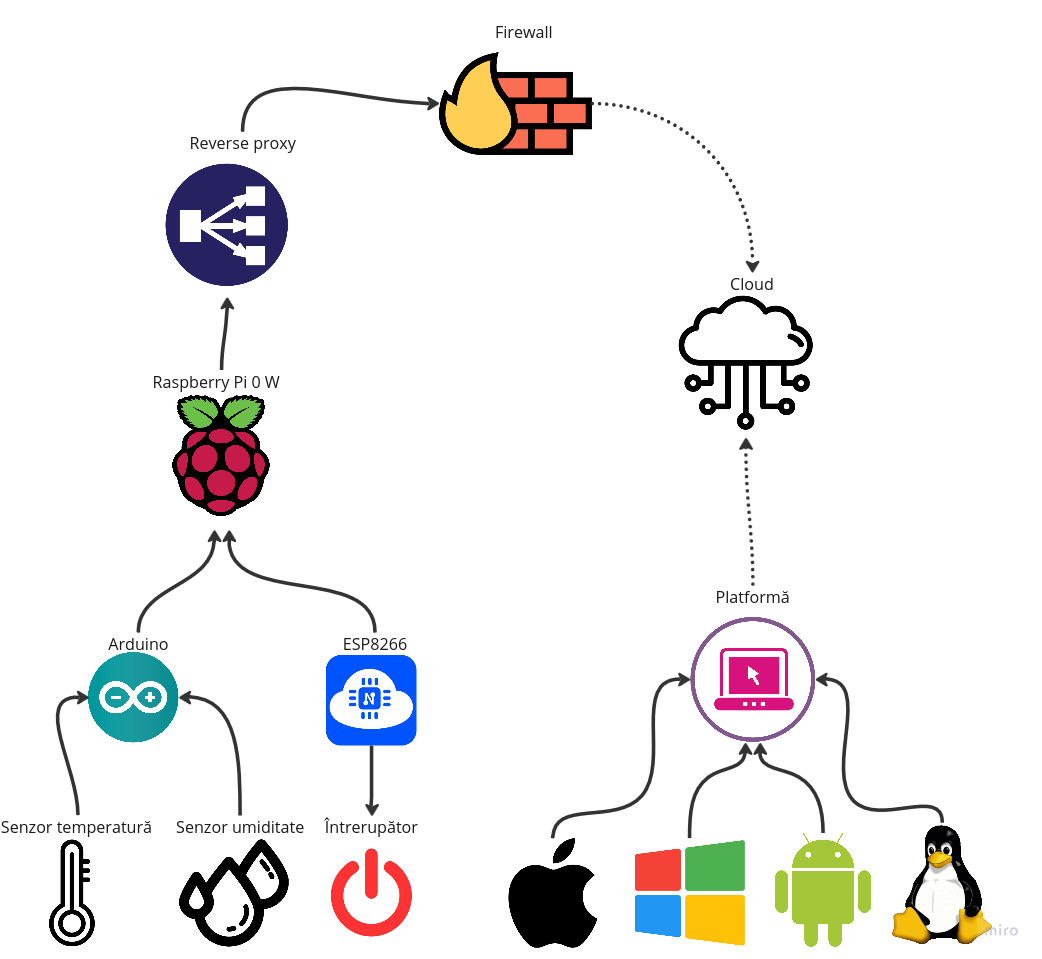
\includegraphics[width=0.7\textwidth]{arhitectura}
	\caption{Legătura dintre componentele soluției}
	\label{fig:arhitectura}
\end{figure}

In imaginea prezentata anterior putem observa un exemplu al arhitecturii aplicatiei si cum sunt legate componentele intre ele. Aceasta aplicatie poate fi utilizata pe platformele: Windows/Mac/Linux/iOS/Android. Ele sunt conectate la senzorii casei prin intermediul serverului care ruleaza pe un Raspberry Pi cu ajutorul API-urilor.

\newpage
\section{Pagina principală}

\begin{wrapfigure}{r}{0.4\textwidth}
	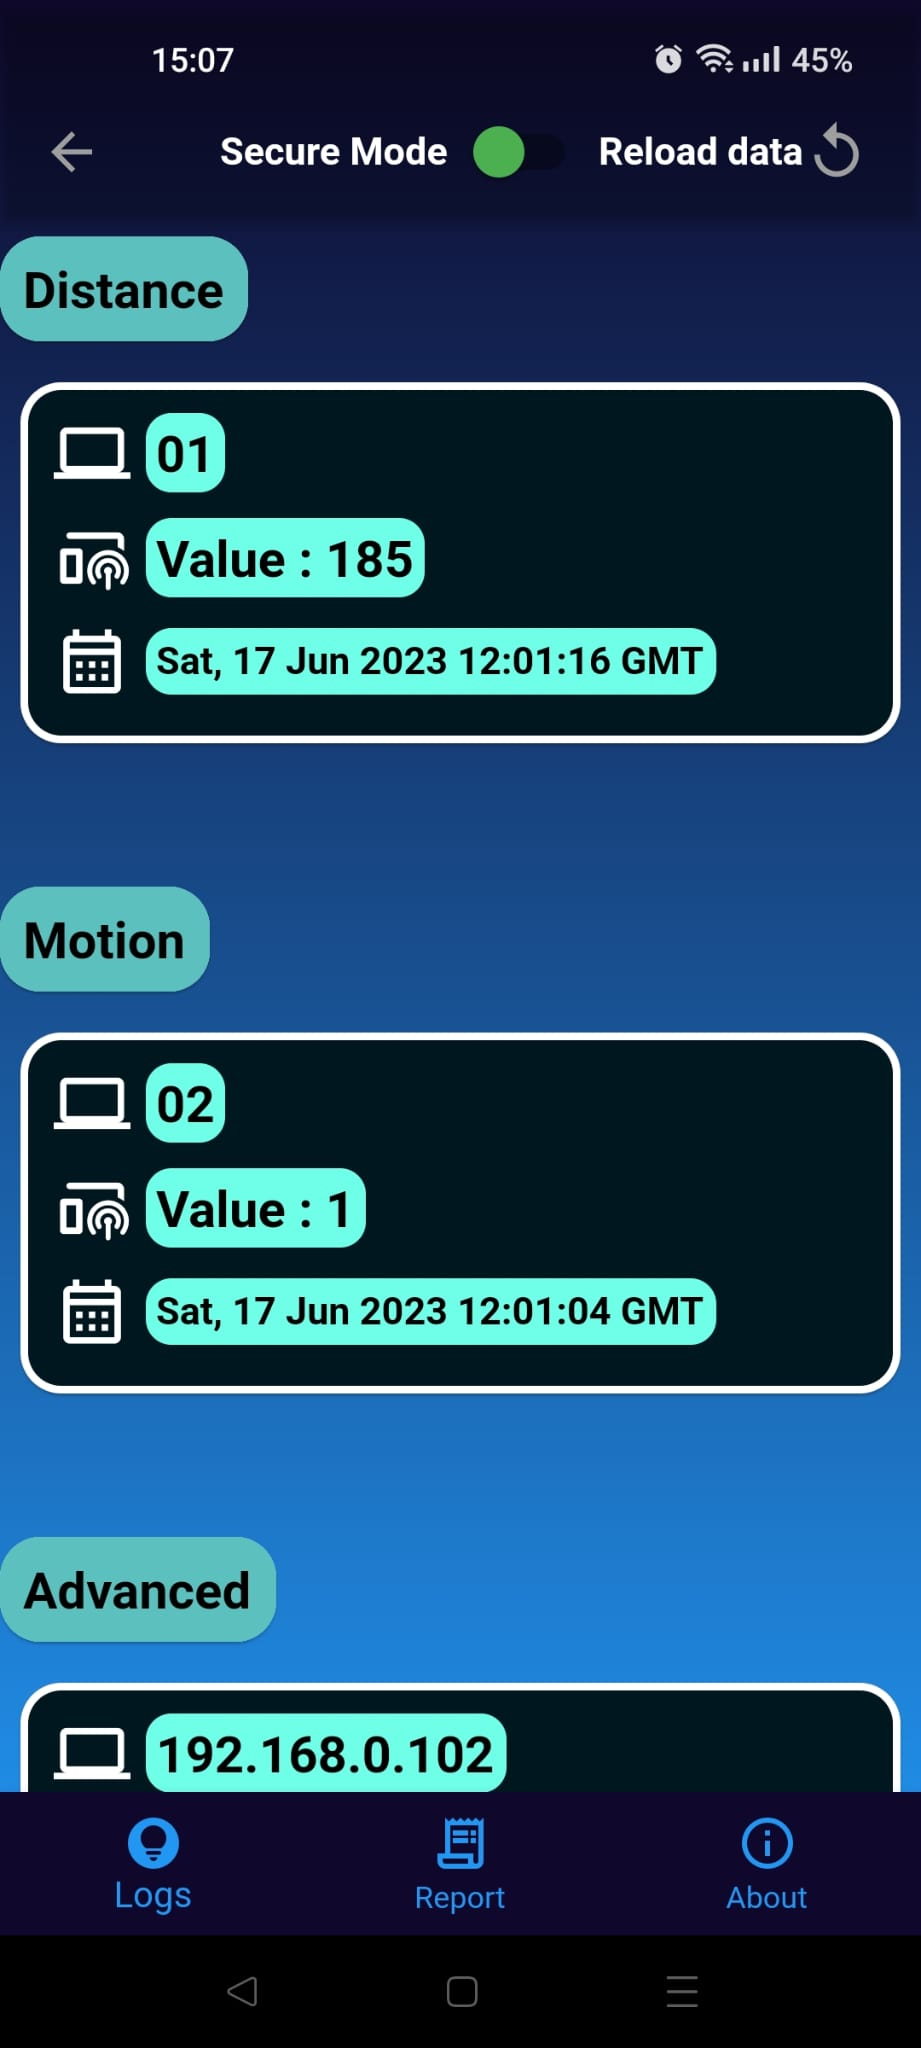
\includegraphics[width=1\linewidth]{1a}
	\caption{Pagina principală}
	\label{fig:1}
\end{wrapfigure}

Primul punct de contact dintre un utilizator și acest proiect este aplicația de telefon (Figura \ref{fig:1}). Odată lansată, va prezenta un splash screen, urmat de pagina principală. Aici se regăsesc toți senzorii conectați la sistem, împreună cu id-ul, valoarea cu timpul la care au fost înregistrate și locația din casă a senzorului. 

Aceștia sunt sortați după parametrul pe care îl colectează, fie detectarea mișcării, calcularea distanței, a temperaturii sau a umidității, lucru care se observă din titlurile situate deasupra fiecărui cartonaș. Aceste device-uri se numesc \emph{senzori statici}, care sunt folosiți doar pentru colectare de informații. Mai există alt tip de senzor numit \emph{dinamic} a cărui caracteristici seamănă cu a celor statici, singura diferență fiind posibilitatea de comunicare bidirecțională. În cazul acestui proiect, singurul senzor de acest tip va închide și deschide o lampă.

În partea de sus se află două butoane, unul de activare/ dezactivare a \emph{modului de securitate} alături de cel de refresh care preia cele mai recente valori ale senzorilor, fiecare având o secțiune dedicată funcționalității și a modului de utilizare.

În partea inferioară a ecranului există alte trei butoane care servesc, în ordine, pe post de \textbf{centru de notificări}, \textbf{generare de rapoarte} și \textbf{informații despre autor}, funcționalitățile fiecăruia fiind detaliate în secțiunile aferente: \ref{section:logs} și \ref{section:report}.

\subsection{Cărțile senzorilor}

Cărțile reprezintă principala sursă de informații pe care un utilizator o regăsește instant când accesează aplicația. Ele oferă date importante despre senzorul respectiv într-o formă ușor de înțeles și de citit rapid.

În prima parte putem observa numele de identificare a senzorului. Acesta îi este asignat manual atunci când placa Arduino este programată și trebuie neapărat să fie unic în toată rețeaua. 

\begin{wrapfigure}{r}{0.4\textwidth}
	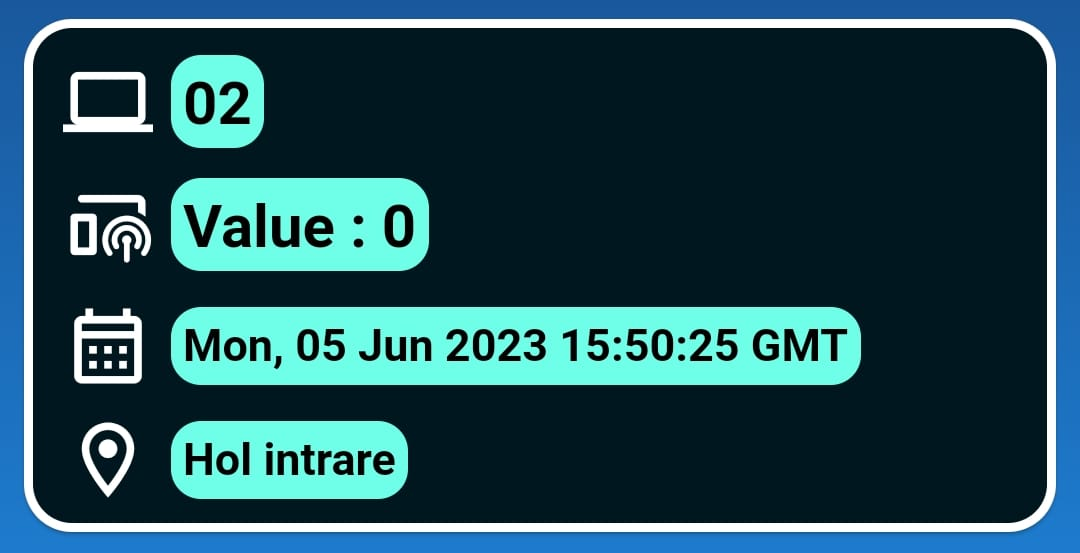
\includegraphics[width=0.5\textwidth]{3}
	\caption{Valorile unui modul}
	\label{fig:3}
\end{wrapfigure}

În cazul în care există multiple dispozitive cu același ID, stația de bază va crede că a primit două pachete de la același senzor, când defapt au fost trimise de către senzori care, foarte probabil, sunt programați să colecteze date diferite și astfel vor apărea discrepanțe vizibile între valorile trimise.

După, putem observa valoarea primită de către aplicație la data și ora respectivă. Odată ce este reîmprospătată pagina, dacă device-ul este conectat la rețea, telefonul va primi cea mai recentă măsurătoare din baza de date care primește informații noi odată la două secunde.

Și nu în ultimul rând, apare și locul fizic exact al senzorului, el fiind setat de către utilizator în aplicație. Inițial, acest câmp nu este vizibil deoarece senzorii nu au atașați un loc predefinit, atașarea și schimbarea lui fiind făcute de către utilizator.

Când vine vorba despre device-urile dinamice, au o interfață asemănătoare, singura diferență fiind câmpul de adresă care deține IP-ul local al senzorului.

Atunci când acest widget este apăsat, utilizatorul va intra pe pagina senzorului respectiv, detaliile căreia vor fi prezentate în secțiunea \ref{section:static}.
\newpage
\subsection{Locația senzorului}

\begin{wrapfigure}{r}{0.4\textwidth}
	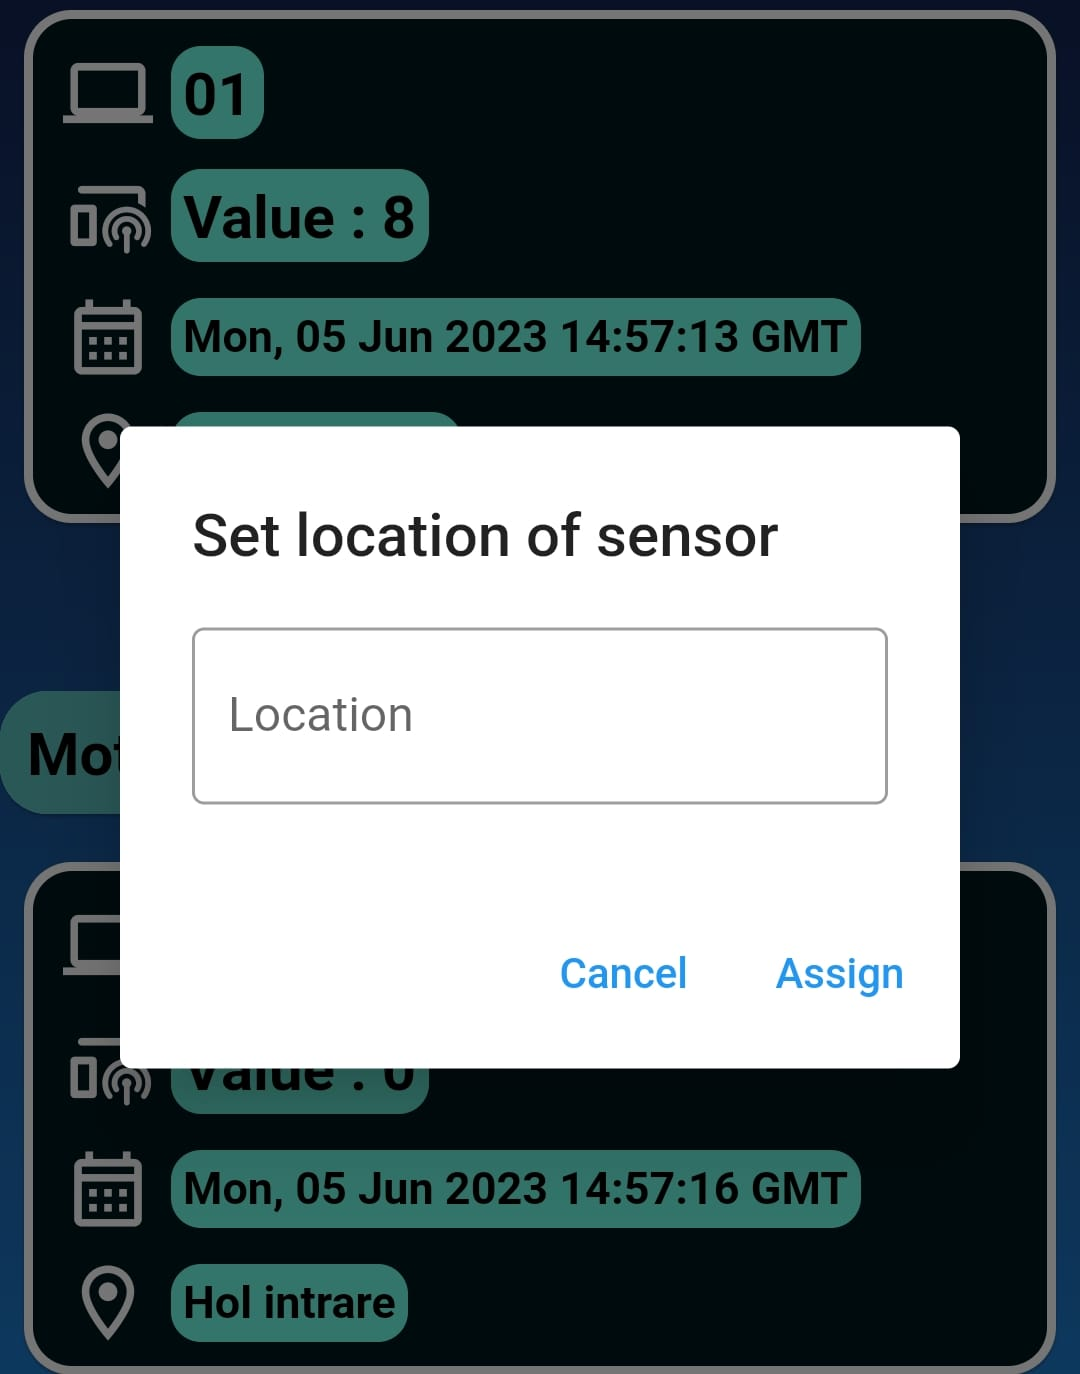
\includegraphics[width=0.4\textwidth]{2}
	\caption{Pop-up pentru locație}
	\label{fig:2}
\end{wrapfigure}
Cu un suport larg de diferite gesturi cu ajutorul clasei GestureDetector din Flutter, avem acces la o suită de detectări a mișcărilor degetetului care pot executa anumite funcții. În cazul aplicației, odată ce se ține apăsat pe un cartonaș, va apărea un dialog în care putem introduce locația fizică a senzorului.
\hfill
Aceasta este salvată în memoria locală a telefonului cu ajutorul bibliotecii de gestionare a bazelor de date NoSQL (non-relaționale). Am ales biblioteca respectivă datorită performanței ridicate, simplitatea oferită și compatibilitatea cross-platform care este critică deoarece aplicația aceasta poate fi compilată pentru majoritatea device-urilor populare. 


\subsection{Modul de securitate} 
\label{section:securitate}

\begin{wrapfigure}{r}{0.4\textwidth}
	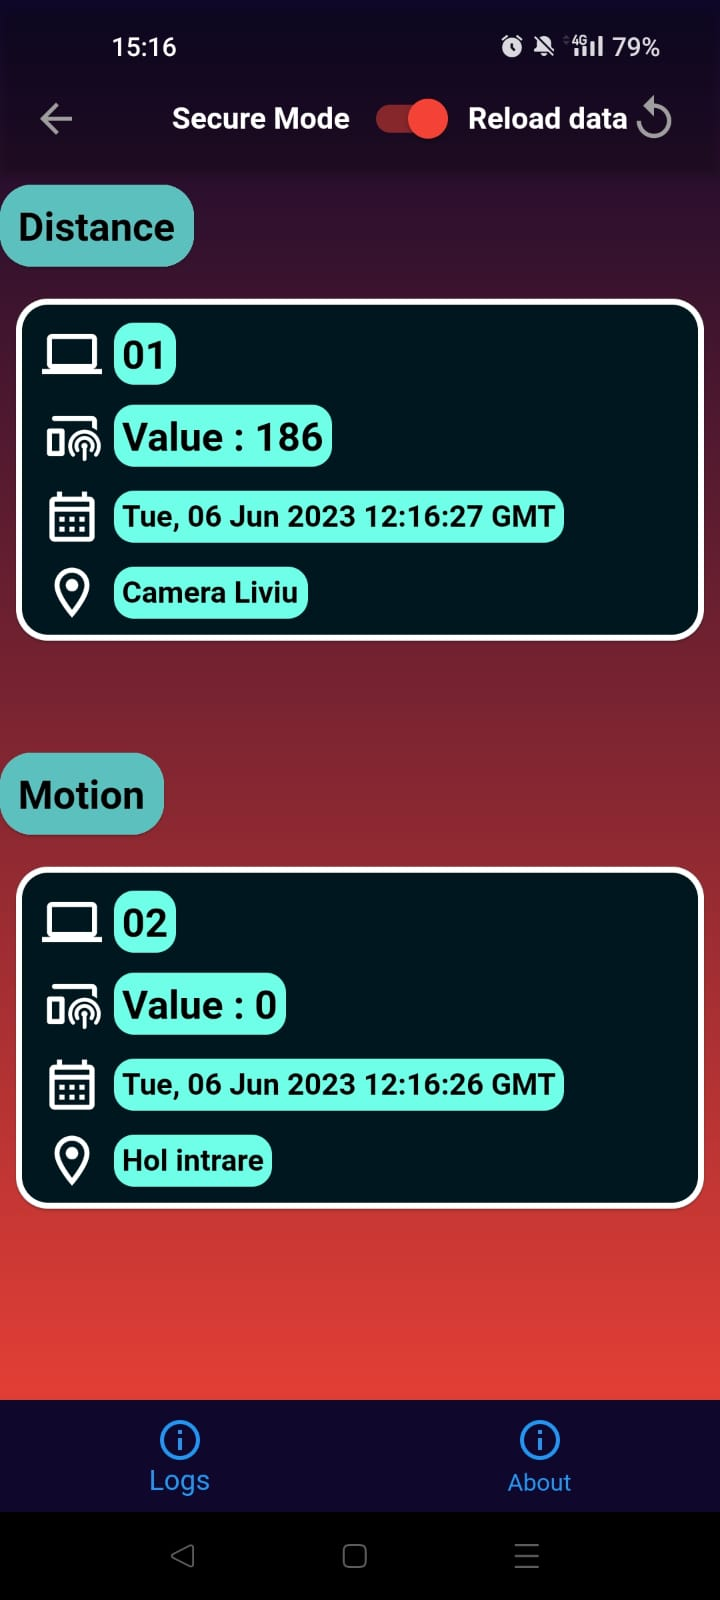
\includegraphics[width=0.3\textwidth]{4}
	\caption{Interfață secure mode}
	\label{fig:4}
\end{wrapfigure}

În ultimii ani, numărul de furturi din locuințe se află pe un trend descrescător, conform informațiilor oferite de către Inspectoratul General al Poliției Române (\textbf{IGPR}). Așadar, în anul 2019 au fost înregistrate 22341 de furturi, iar în 2020 infracțiunile au ajuns la 18060, cu 19\% mai puține față de anul precedent. Chiar și în aceste circumstanțe, acest număr se datorează mentalității defensive în continuă dezvoltare și a sistemelor de alarmă care devin tot mai sofisticate. Am decis că introducerea unei astfel de abilități va contribui pozitiv la securizarea locuinței în care sistemul este instalat.

Modul de securitate se încadrează la categoria de bariere \emph{psihice} deoarece \emph{"descurajează infractorii sau detectează în faza incipientă o tentativă de pătrundere prin efracţie (sisteme de securitate perimetrală, antiefracţie, control al accesului sau sisteme de supraveghere şi înregistrare video)"}\footnote{\url{https://www.politiaromana.ro/ro/prevenire/furturi-din-locuinte}.}

Este recomandat ca, atunci când utilizatorul pleacă din incinta în care este instalată soluția smart home, să activeze modul de securitate. Fiecărui senzor îi poate fi atribuit o limită astfel încât orice valoare preluată  care scade sub acest prag (numit și \emph{Threshold}), va apărea sub forma unei notificări pe pagina de \emph{Logs}.

După ce este activat, utilizatorului îi este făcut prezent acest fapt prin schimbarea culorii de background. Valoarea acestui buton este salvată în baza de date Hive, împreună cu data și ora la care a fost schimbată. Aceasta din urmă va fi folosită la filtrarea alarmelor false.

Senzorii dinamici pot fi configurați astfel încât să se folosească de această valoare și din acest motiv, la fiecare schimbare a acestui buton, valoarea va fi postată pe ruta \textbf{https://andr3w.ddns.net/secure}, urmând să fie disponibilă tuturor device-urilor pentru a o putea citi.

\subsection{Butonul de refresh}

Funcționalitatea sa este intuitivă, întrucât apăsarea lui rezultă în re-împrospătarea valorilor din aplicație cu cele mai recente citiri ale tuturor senzorilor sistemului. Deoarece tot backend-ul este hostat pe un procesor cu un singur nucleu, am decis să implementez o metodă de \emph{caching} a datelor pentru sesiunea curentă. În acest mod salvăm serverul de la multe request-uri și economisim datele mobile.

Una din limitările sistemului este că informațiile afișate nu sunt actualizate constant. Acest lucru duce la discrepanțe între valorile pe care utilizatorul le vede și cele pe care senzorii le trimit. Vom vorbi despre aceasta în capitolul dedicat viziunii pe viitor.

\break

\section{Pagina senzorului static}
\label{section:static}

\begin{wrapfigure}{r}{0.3\textwidth}
	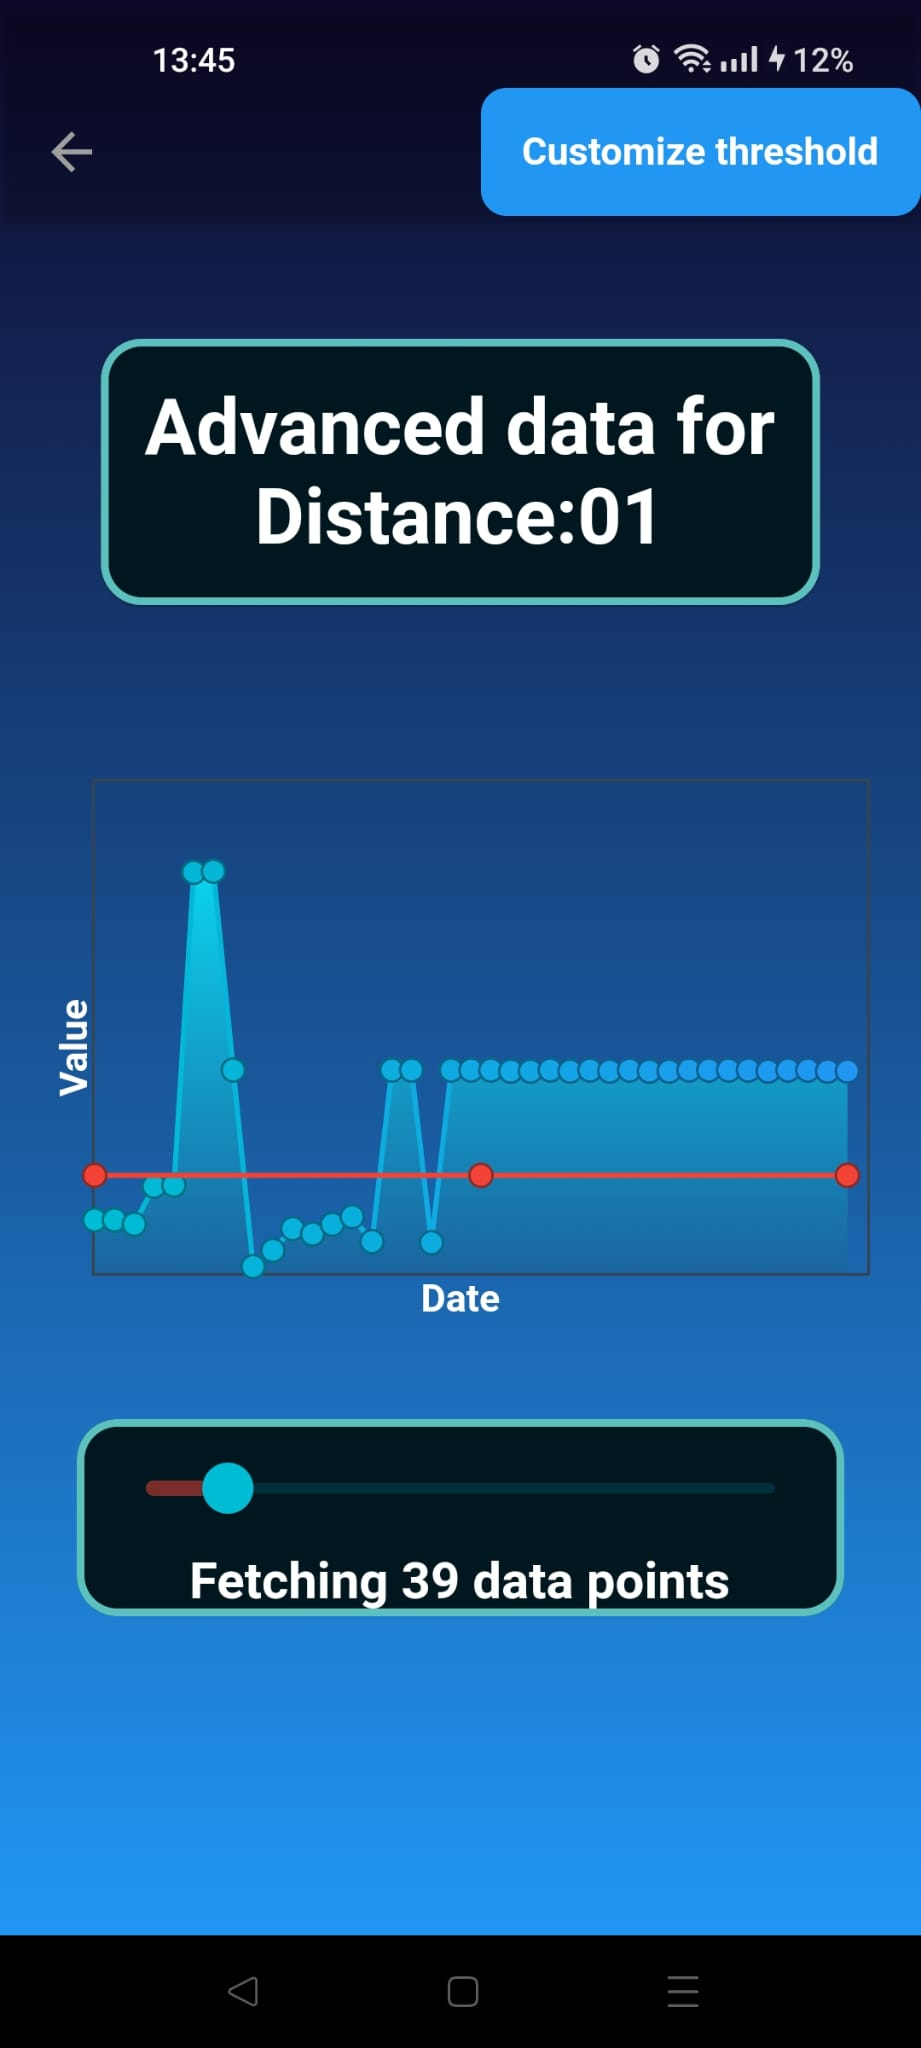
\includegraphics[width=0.4\textwidth]{5}
	\caption{Date avansate despre senzorul 01}
	\label{fig:5}
\end{wrapfigure}

Pe această rută se află informații și setări care contribuie la sensul de Smart home: componente ce lucrează împreună pentru a aduce utilizatorului un aport esențial de securitate.

AppBar-ul este populat cu un buton de setare a unei limite, valoare despre care am vorbit în secțiunea \ref{section:securitate}. Odată ce \emph{threshold} este setat (Figura \ref{fig:5}), va fi salvată în baza de date locală, astfel ea persistând chiar și când restartăm aplicația. Ca să fie vizibilă utilizatorului, pe graficul de mai jos se va trasa o linie roșie (care nu există dacă nu avem o limită). Ca utilizare, limita va fi folosită la notificările de pe pagina de \emph{Logs} pentru a determina dacă o înregistrare trebuie arătată utilizatorului în caz că valoarea ei scade sub limita asignată.

În prim plan se află graficul care afișează evoluția ultimelor N înregistrări ale senzorului respectiv în funcție de data la care au fost colectate individual. Fiindcă sunt foarte multe puncte afișate, nu am putut include vizual și valorile lor, dar, utilizatorul o poate vedea, împreună cu data aferentă dacă apasă pe oricare punct (Figura \ref{fig:6}). Pentru construcția sa, am decis să folosesc librăria \textbf{fl\_chart} datorită popularității și a documentației excelente. Este un grafic fluid deoarece odată ce se modifică valorile afișate, motorul fl\_chart creează o animație de tranziție de la informațiile vechi la cele noi.

Dedesubtul figurii apare un slider care setează numărul de puncte extrase de la server. A existat o problemă aici care îmi făcea un API call la fiecare schimbare de valoare, adică dacă de la 39 de puncte doresc să îmi afișeze 200, va face 200-39 = 161 request-uri către backend. Remediul a fost ca reîmprosătarea să fie făcută în funcția \textbf{onChangeEnd} care va trimite cererea către server atunci când s-a terminat de ales cantitatea de informații, evitând astfel un \emph{Denial of Service} pentru server.

\begin{figure}[h]
	\centering
	\begin{subfigure}{0.4\textwidth}
		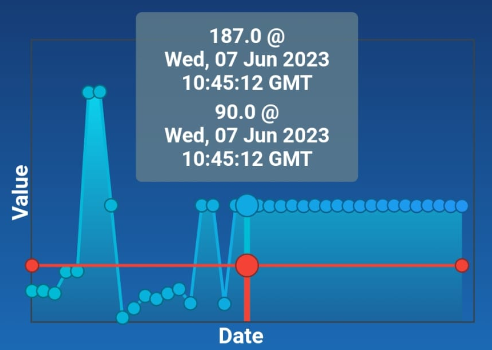
\includegraphics[width=\textwidth]{6}
		\caption{Grafic}
		\label{fig:6}
	\end{subfigure}
	\hfill
	\begin{subfigure}{0.4\textwidth}
		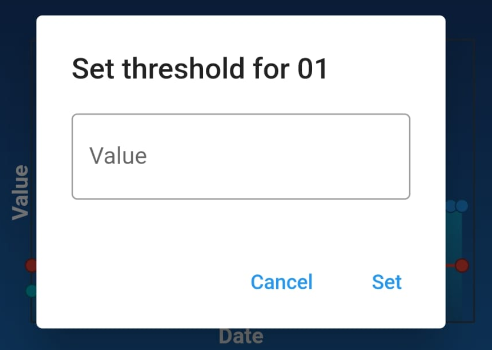
\includegraphics[width=\textwidth]{7}
		\caption{Dialog limită}
		\label{fig:7}
	\end{subfigure}
	\caption{}
	\label{fig:all3}
\end{figure}

\section{Pagina senzorului dinamic}

\begin{wrapfigure}{r}{0.3\textwidth}
	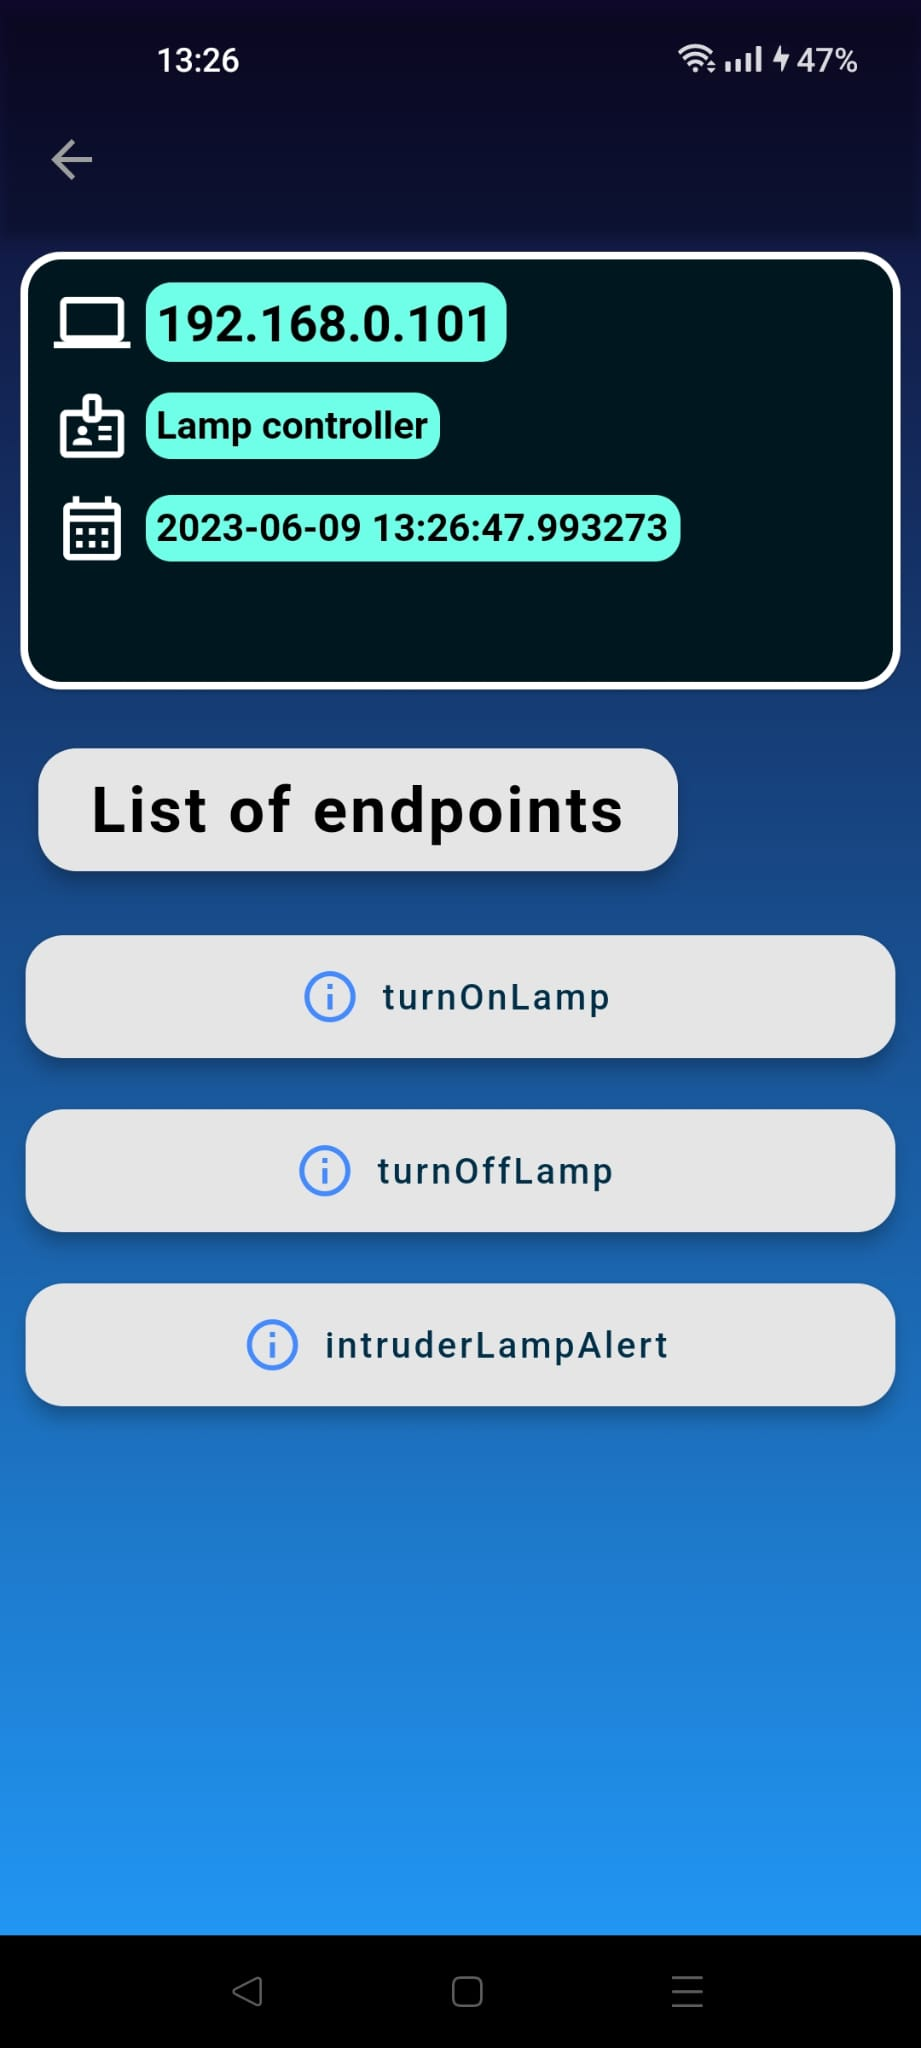
\includegraphics[width=0.4\textwidth]{8}
	\caption{Informații și rutele senzorului dinamic}
	\label{fig:8}
\end{wrapfigure}

Modulele dinamice sunt destul de diferite față de cele statice, întrucât se conectează direct la rețeaua locală de Wi-Fi (fiindu-le asignat o adresă IP) și pot primi sau trimite comenzi la server sau la alte module dinamice. M-am decis să adaug acest tip de senzori datorită recomandării îndrumătorului licenței, domnul profesor Vidrașcu, o adiție ce se pliază perfect pe subiectul abordat în această teză: \textbf{o soluție smart home orientată pe confidențialitate}.

După cum se poate observa, avem afișate datele despre senzor într-o manieră similară cu cea de la cei statici, diferența fiind IP-ul. Senzorii dinamici pot fi controlați de către utilizator și, în acest caz, este prin intermediul butoanelor ce apelează \emph{endpoint-urile} hostate pe ESP8266. Un endpoint reprezintă o locație către care se pot face cereri HTTP (GET, POST, PUT, DELETE) pentru a manipula resursele unui serviciu. Serverul de pe ESP8266 își publică endpoint-urile la stația de bază care arată astfel: \textbf{http://192.168.0.101/turnOffLamp}. Fiecare rută pe care o apelăm va instrui senzorul să execute diferite funcționalități care pot fi deduse din numele afișat pe buton. \textbf{IntruderLampAlert} desemnează cum reacționează acest modul atunci când modul de securitate este activat și senzorul de mișcare emite un ”1” logic.

\section{Pagina de informații}
\label{section:logs}

Fiecare anomalie din sistem (orice senzor ce înregistrează o valoare care a scăzut sub limita impusă) va crea o notificare pe care utilizatorul o poate verifica în secțiunea de \textbf{Logs}. Aceasta poate fi accesată din bara de footer al meniului principal.

\begin{figure}[h]
	\centering
	\begin{subfigure}{0.45\textwidth}
		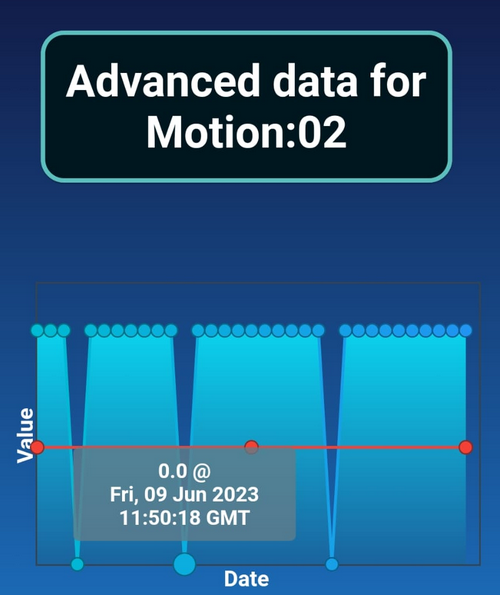
\includegraphics[width=\textwidth]{11}
		\caption{Valori ce vor genera erori}
		\label{fig:11}
	\end{subfigure}
	\hfill
	\begin{subfigure}{0.35\textwidth}
		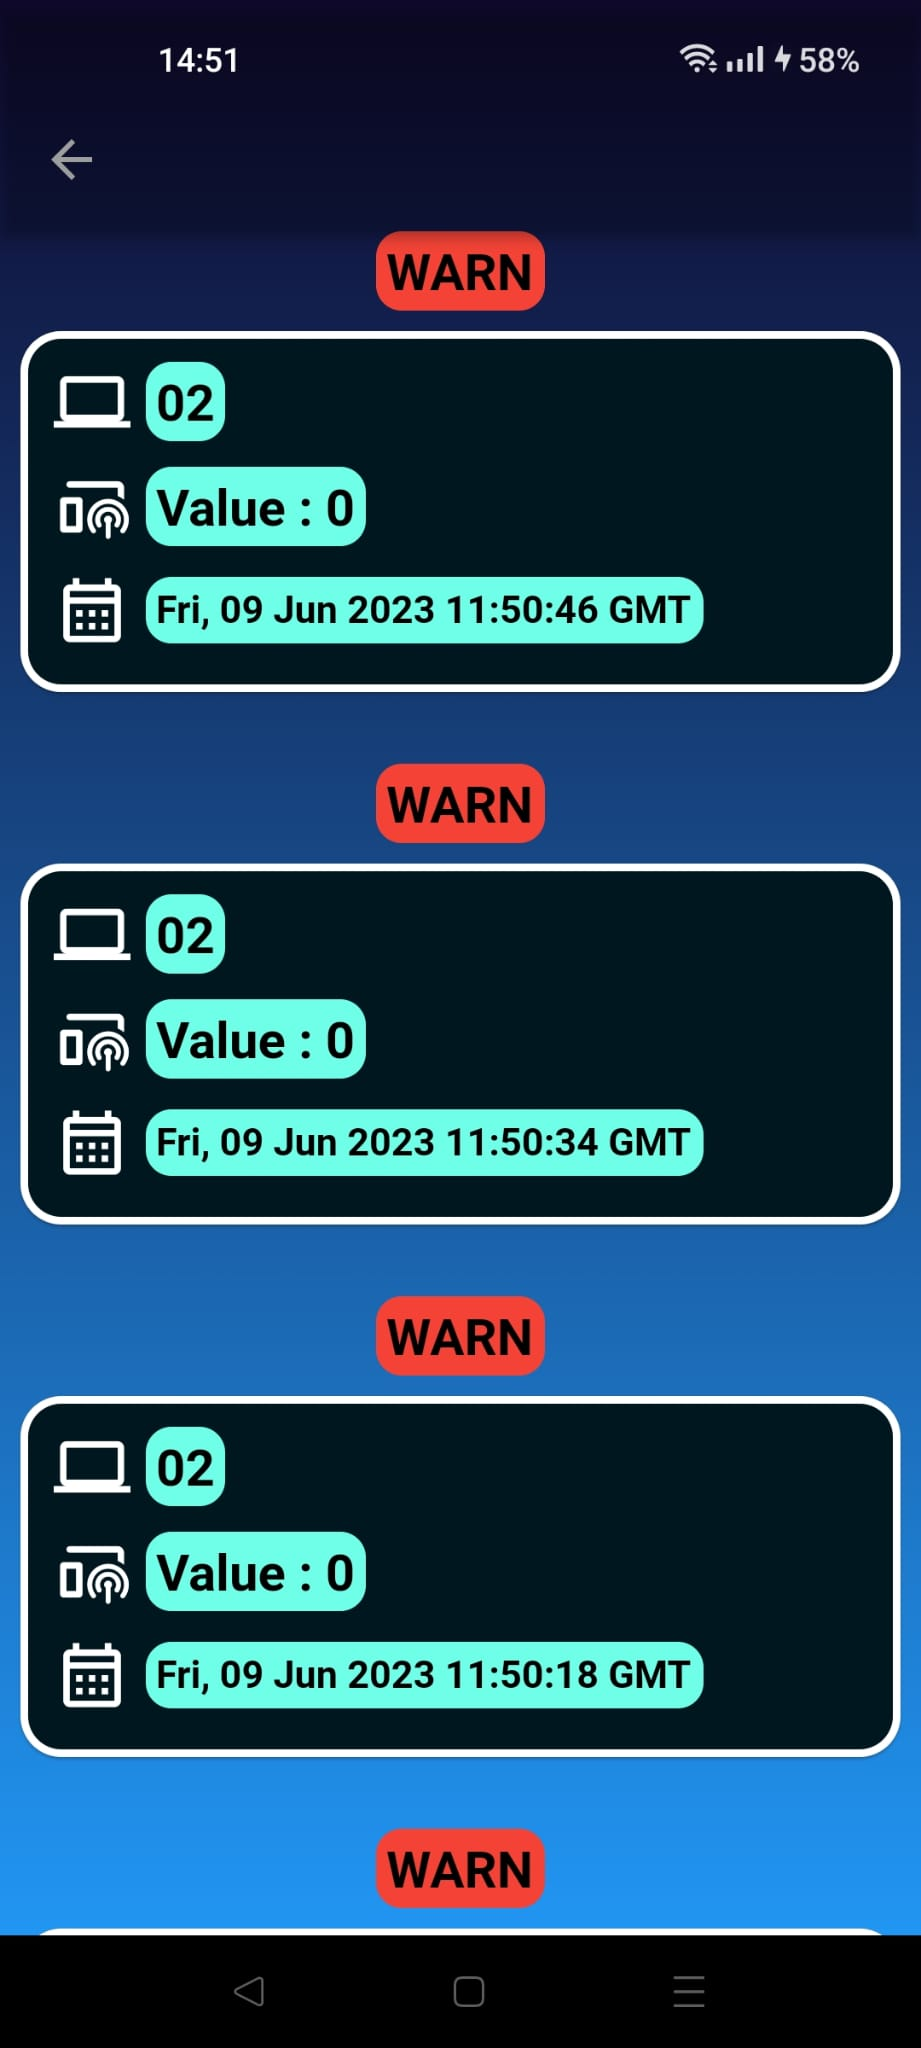
\includegraphics[width=\textwidth]{12}
		\caption{Pagina de logging}
		\label{fig:12}
	\end{subfigure}
	\caption{}
	\label{fig:all5}
\end{figure}

Inițial, aplicația nu generează notificări dacă un senzor a înregistrat o abatere de la normal atunci când \textbf{Secure Mode} nu este activat deoarece se presupune că utilizatorul nu a plecat încă de acasă. Activarea modului de securitate va cauza afișarea anomaliilor pe ecran.

Din figura \ref{fig:11} se pot extrage anumite informații astfel: există trei puncte care se află sub bariera setată cu ajutorul butonului \textbf{Set threshold}, ceea ce înseamnă că utilizatorul și-a părăsit apartamentul, dar încă există activitate. 

Aplicația va prelua ultimele înregistrări a fiecărui senzor pe care le compară cu limita (stocată în baza de date locală) și afișează cartonașele corespunzător. Se poate observa în figura \ref{fig:12}. că ultima alertă este cea din figura anterioară.

\break

\section{Pagina de generare de rapoarte}
\label{section:report}

În cazul în care utilizatorul este o victimă a unui jaf sau unei intruziuni în casă, este important să acționeze în mod corespunzător. Primul pas este să își asigure siguranța personală și să sune imediat la serviciile de urgență sau la poliție, încercând să nu intre în contact cu posibilii infractori sau să manipuleze evidențele rămase la fața locului, pentru a nu distruge potențiale probe. După anunțarea autorităților, trebuie făcută o inventariere a obiectelor pierdute și să fie extrase cât mai multe informații din ziua respectivă legate de incident.

Aplicația din această soluție ajută utlizatorul în cazul unui astfel de eveniment prin colectarea tuturor datelor senzorilor din casă, expunându-le în formă de PDF gata să fie oferite autorităților. Trebuie menționat faptul că senzorii au fost plasați specific în holul de la intrarea în apartamentul meu, pozitionați astfel încât orice persoană care intră va modifica starea modulelor.

Interfața (Figura \ref{fig:9}) este alcătuită din cele două câmpuri ce permit introducerea timpului de început și cel de sfârșit. Acestea vor fi folosite de către server pentru a filtra toate înregistrările senzorilor, luându-le doar pe cele ce se încadrează în intervalul specificat. Cele două valori trebuie neapărat setate, întrucât butonul de \textbf{Generate report} nu va funcționa fiindcă nu știe unul din capetele intervalului sau chiar ambele. Odată apăsat, va trimite un POST request la stația de bază care îi va răspunde cu datele aferente. Utilizatorul este notificat de terminarea procesului printr-un pop-up în josul ecranului ce oferă și folderul în care a fost salvat.

Cu ajutorul librăriei \textbf{pdf} din cadrul SDK-ului Flutter, am reușit generarea documentului (Figura \ref{fig:10}). Pe post de header, am specificat intervalul din care au fost extrase informațiile senzorilor și data la care a fost creat acest document. Footer-ul conține numele aplicației și deținătorul drepturilor licenței. În centrul atenției este un tabel ce conține, în ordine, numărul curent al înregistrării, adresa, data, ID-ul, tipul și valoarea senzorului. Acesta este extins pe multiple foi, cifra din partea de jos al ecranului desemnând numărul curent al paginii. Pentru raportul acesta avem un număr de 300 de înregistrări preluate în decursul a 5 minute. Stația de bază este responsabilă să recepționeze și să citească pachetele trimise de toți senzorii, lucru care devine destul de greu atunci când fiecare device transmite în aceeași secundă după cum se observă în PDF. Datorită librăriei \textbf{RF24Network} despre care vom vorbi în secțiunea senzorilor statici, toate pachetele vor fi decodate cu succes.

Datele acestui document sunt valoroase și pot ajuta foarte mult investigatorii, crescând astfel șansele de a prinde intrușii. Asigurând proprietarii ce folosesc acest sistem cu un raport plin de informații, soluția de smart home propusă joacă un rol important în creșterea securității utilizatorului.

\begin{figure}[h]
	\centering
	\begin{subfigure}{0.43\textwidth}
		\centering
		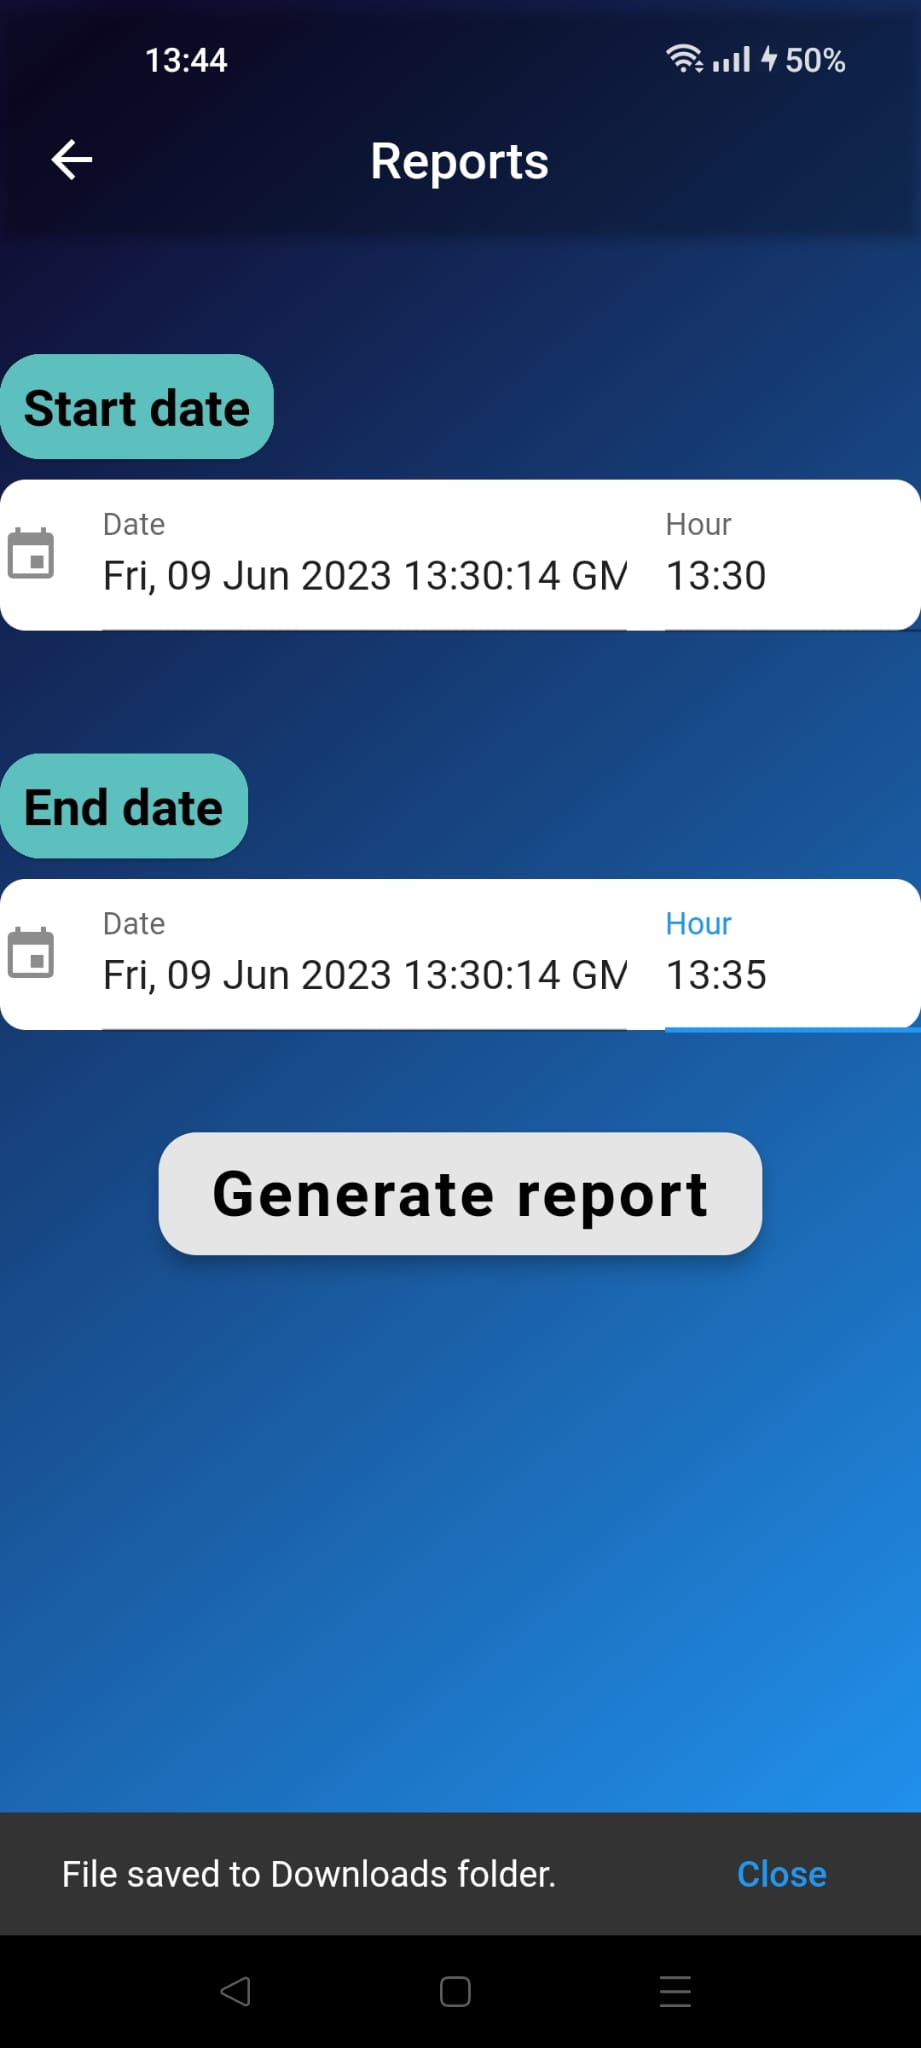
\includegraphics[width=\textwidth]{9}
		\caption{Interfața paginii}
		\label{fig:9}
	\end{subfigure}
	\hfill
	\begin{subfigure}{0.43\textwidth}
		\centering
		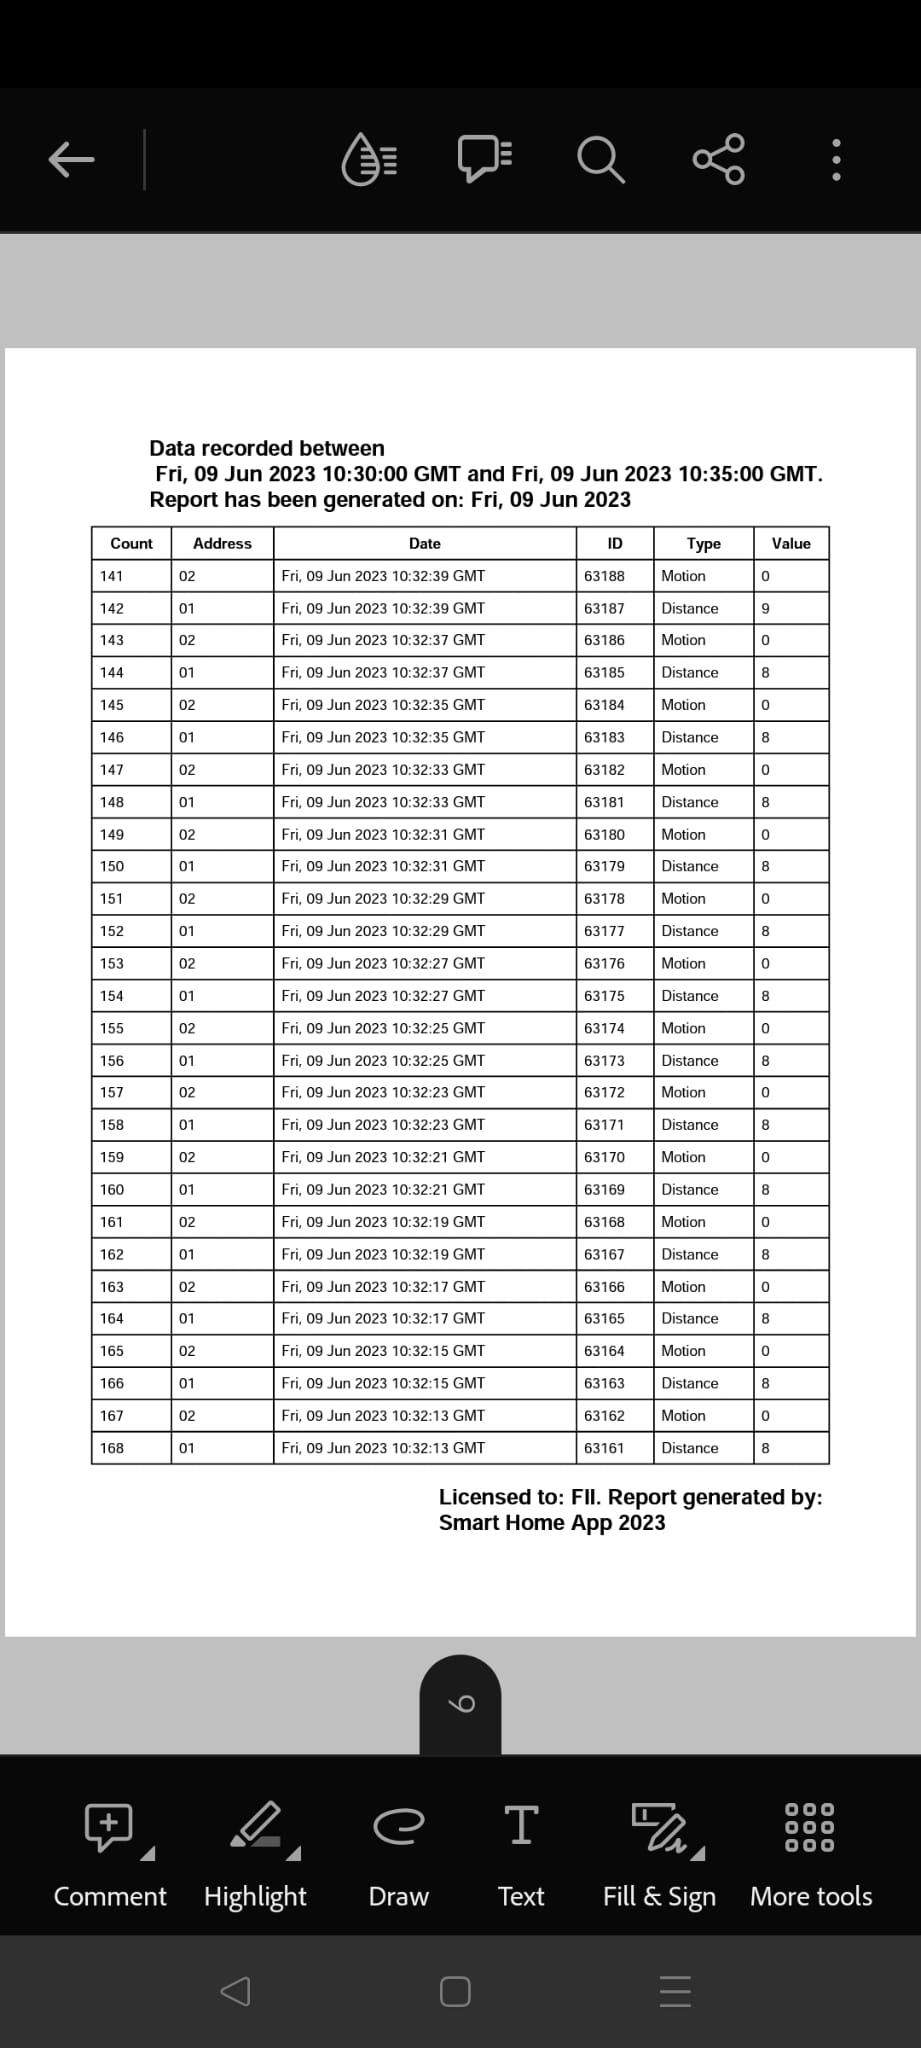
\includegraphics[width=\textwidth]{10}
		\caption{PDF-ul generat}
		\label{fig:10}
	\end{subfigure}
	\caption{}
	\label{fig:all4}
\end{figure}
\break


\section{Modul debug}

\textbf{Network\_rx.py} reprezintă modul de debug, fiind o unealtă care ajută utilizatorul la momentul instalării senzorilor sau atunci când unii nu mai funcționează corespunzător.

În timpul execuției, acesta afișează în consolă (Figura \ref{fig:13}) toate pachetele pe care le primește în timp real. Acest lucru este util deoarece permite utilizatorului să confirme că senzorii funcționează corect și trimit datele corespunzătoare. Problemele de comunicare sunt depistate din timp, de obicei acestea se rezolvă cu o restartare a modulelor.

Fiecare linie deține datele unei înregistrări: \textbf{payload len} reprezintă lungimea în octeți a pachetului, \textbf{sensor type} e tipul senzorului (distanță, temperatură, mișcare), \textbf{value} conține valoarea citită de device, iar \textbf{header} are date precum id-ul pachetului, emițătorul și receptorul, care în cazul acesta este stația de bază la adresa \textbf{00}.

\begin{figure}[h]
	\centering
	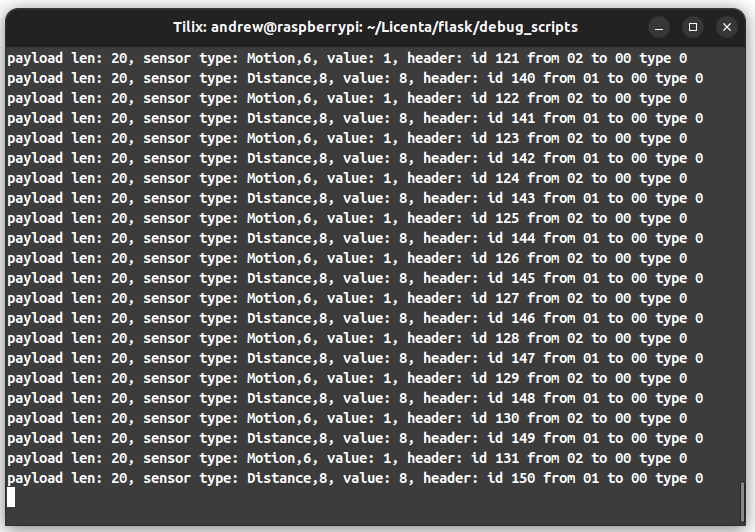
\includegraphics[width=0.6\textwidth]{13}
	\caption{Detaliile senzorilor conectați la stația de bază}
	\label{fig:13}
\end{figure}

Este important ca user-ul să aibă instalate toate librăriile de care acest script depinde, lucru despre care vom intra în detaliu la secțiunea backendului. Fiind un script scris în python aflat în folderul \textbf{debug\_scripts}, este executat prin introducerea comenzii \textbf{python3 Licenta/flask/debug\_scripts/network\_rx.py}. Fiindcă rulează la infinit, se poate ieși din el apăsând \textbf{Ctrl + C} sau urmând instrucțiunile de aici. \footnote{\url{https://github.com/hakluke/how-to-exit-vim\#the-hardware-way}}

\newpage

\section{Frontend}

Înainte de a intra în detaliu la fiecare element, este important de a înțelege că Flutter deține o gamă largă de elemente și componente care formează bazele unei interfețe grafice, noțiunile pe care le-am folosit în acest proiect fiind de dificultate medie.

Printre aceste elemente, regăsim:
\begin{itemize}
	\item Scaffold: este unul din componentele fundamentale din acest \emph{SDK}, oferindu-ne o suprafață pe care o putem popula cu \textbf{AppBar} sau \textbf{BottomNavigationBar};
	
	\item Column și Row: sunt widget-uri pentru îmbunătățirea aspectului. Elementele ce vor fi poziționate în ele vor fi aranjate vertical, respectiv orizontal;
	
	\item FloatingActionButton: reprezintă un buton care, odată apăsat, va notifica sistemul să execute funcția sa asociată;
	
	\item AppBar: este elementul vizual care acționează pe post de Header al aplicației, se îmbină de obicei cu Scaffold;
	
	\item FutureBuilder: această componentă va construi în mod concurent elemente de interfață care sunt extrase de la API-uri.
\end{itemize}

\section{REST API}

Un \textbf{API} (\textbf{Application programming interface}) este un mecanism care permite unui serviciu să acceseze resursels unui alt serviciu. REST API se bazează pe principii precum utilizarea verbelor HTTP (GET, PUT, POST, DELETE) pentru transmiterea și manipularea datelor într-un format standardizat (XML, JSON), împreună cu ajutorul \textbf{URI} (uniform resource identifier) pentru specificarea resursei asupra cărei operațiile vor fi executate. Am creat astfel o arhitectură REST pentru a servi diferite informații către aplicația de mobil, afișându-le într-o manieră ușor de înțeles \cite{rest}.

Serverul expune rute de accesare a informațiilor din baza de date pentru ambele tipuri de senzori: cei statici se află la adresa \textbf{https://andr3w.ddns.net/ $<$rută$>$}, iar cei dinamici la \textbf{https://andr3w.ddns.net/advanced/$<$rută$>$}

\subsection{DNS dinamic}

Provider-ul de internet asignează dinamic adresele IP utilizatorilor conectați, motiv pentru care după o pană de curent, de obicei se resetează această adresă. Pentru a rezolva această problemă, am utilizat serviciul gratuit de \textbf{Dynamic DNS}\cite{noip} al companiei \textbf{No-IP}\footnote{\url{https://www.noip.com/}}. Setările au fost realizare direct pe router-ul personal, un \textbf{TP-Link WR740N}. Odată configurat, rețeaua locală poate fi accesată de la adresa \url{https://andr3w.ddns.net}.

\section{Backend}

Backend-ul reprezintă partea aplicației responsabilă de logică și funcționalitate. În contextul acestei licențe, am decis să folosesc limbajul \textbf{Python} versiunea 3.10 cu microframework-ul \textbf{Flask} către care sunt trimise pachetele de la \textbf{gunicorn} și \textbf{nginx}.

\begin{figure}[h]
	\centering
	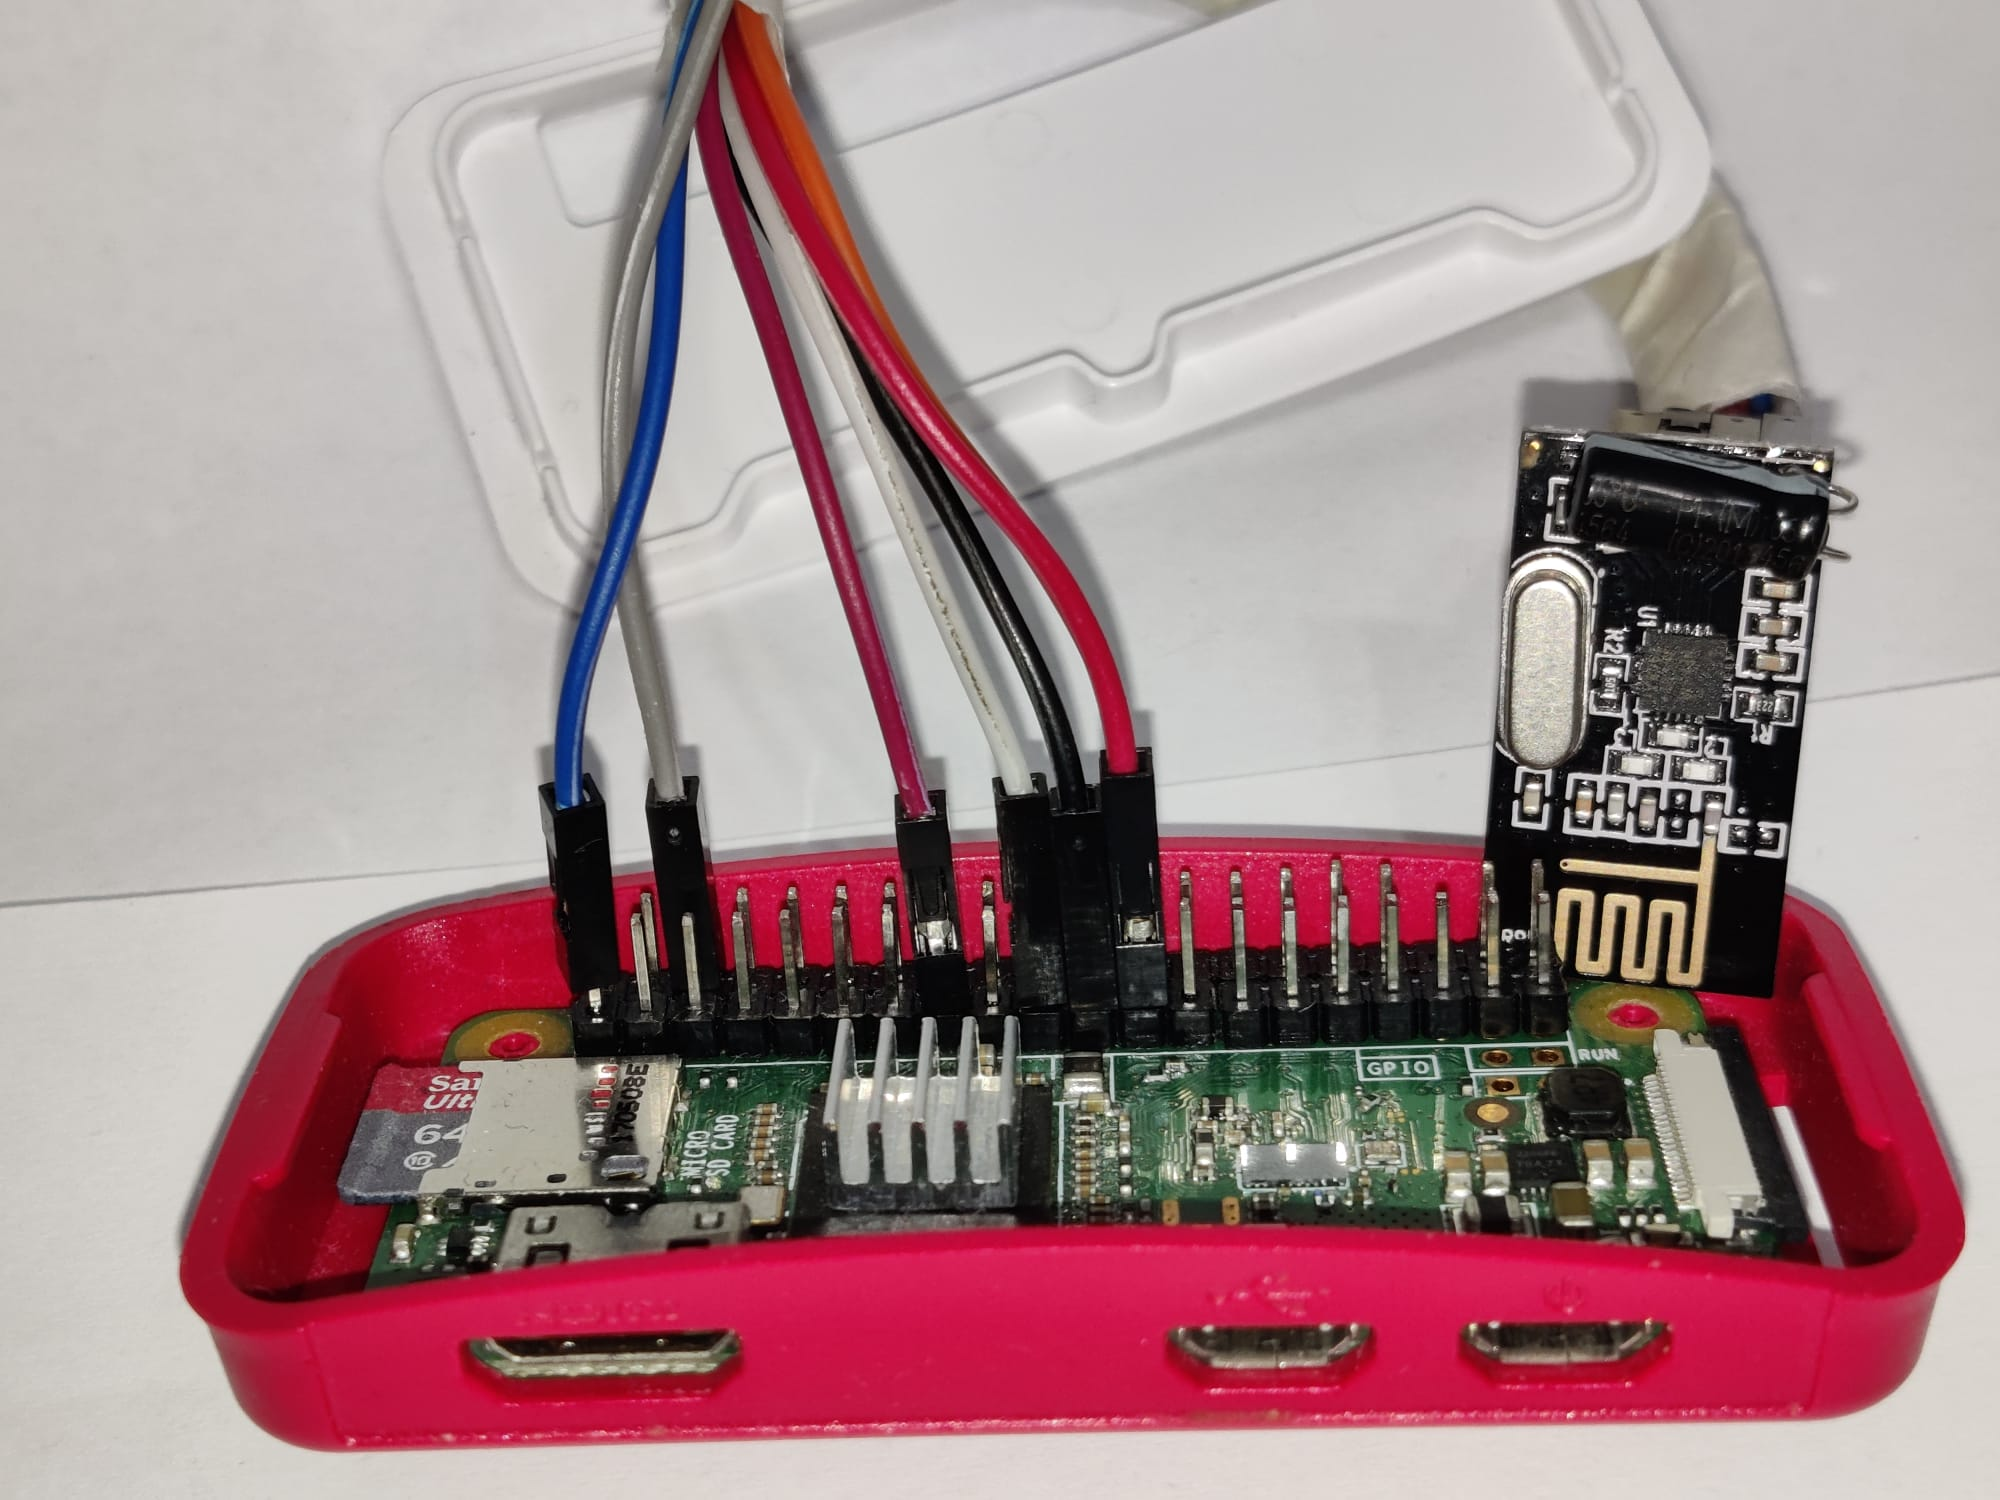
\includegraphics[width=0.65\linewidth]{17}
	\caption{Placa Raspberry ce găzduiește serverul}
	\label{fig:17}
\end{figure}

Acesta rulează pe stația de bază (Figura \ref{fig:17}) pentru a satisface fiecare cerere a utilizatorului, fără a fi nevoit să își deschidă calculatorul personal pentru a putea interacționa cu dispozitivele sale. 

Pentru o productivitate crescută, am ales să instalez sistemul de operare \emph{Raspberry Pi OS Lite} deoarece este rapid, lucru datorat lipsei unei interfețe grafice și a programelor pre-instalate. Instalarea a fost foarte ușoară, urmând instrucțiunile din documentația lor\footnote{\url{https://www.raspberrypi.com/documentation/}}.

Comunicarea cu placa a fost făcută doar prin \textbf{SSH} care a fost deschis din setările router-ului. Fiindcă această conexiune va fi publică, am instalat programul \textbf{ufw} (\emph{uncomplicated firewall}) ce mi-a ușurat securizarea host-ului, fiind o unealtă ce înlocuiește setările complicate ale \textbf{iptables} \cite{iptables} cu comenzi simple: \emph{sudo ufw allow 22}. Astfel am limitat numărul de conexiuni la portul 22 și am permis accesul la portul 443, acestea fiind singurele  căi de acces.

Nginx este un \textbf{reverse proxy} \cite{nginx} care se află între client și backend. Acesta primește cererile din exterior pe care le redirecționează serverului de gunicorn după setările din figura \ref{fig:16}.

Criptarea traficului e realizată direct de către nginx, specificând locația certificatului și a cheii private cu ajutorul comenzilor \emph{ssl\_certificate} și \emph{ssl\_certificate\_key}. Am decis să îmi semnez propriul \textbf{certificat SSL} (Secure sockets layer) cu utilitarul \textbf{openssl}.

\begin{figure}[h]
	\centering
	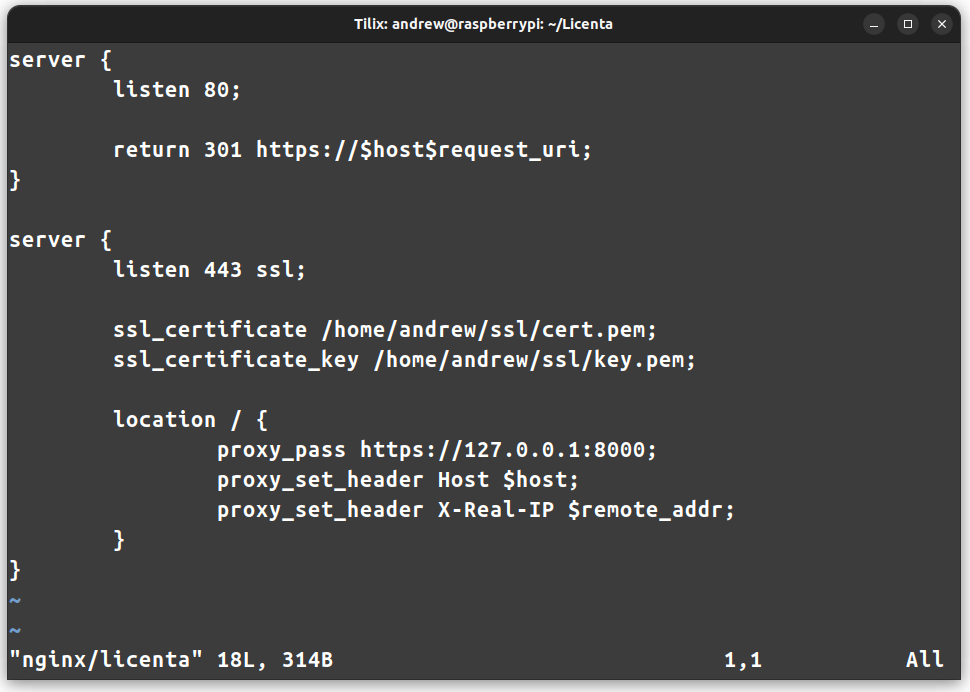
\includegraphics[width=0.65\linewidth]{16}
	\caption{Configurare Nginx}
	\label{fig:16}
\end{figure}

Prima componentă numită \emph{server} interceptează fiecare cerere HTTP pe care o redirecționează la ruta de HTTPS asignată portului 443, returnând astfel codul 301 ce notifică utilizatorul că a fost redirectat de la ruta \textbf{http://} la cea de \textbf{https://}.

A doua componentă asultă la portul 443 (HTTPS) și, datorită blocului \textbf{location /}, orice cerere va fi redirecționată către serverul Flask, fiind configurat a primi request-uri la portul 8000. Trebuie menționat faptul că ambele aplicații rulează pe același host, ceea ce face posibilă trimiterea cu succes către adresa de \emph{loopback}\footnote{\url{https://study-ccna.com/loopback-interface-loopback-address/}}. Această utilizare este ideală deoarece ne aflăm la o scară de nivel de proiect personal. Pentru uz în producție se recomandă folosirea unui proxy server\footnote{\url{https://browserjet.com/blog/advantages-and-disadvantages-of-a-proxy-server}} pe un computer separat.

\subsection{Stocarea datelor}

\textbf{SQLAlchemy} este o colecție de unelte ce ajută programatorul să acceseze și manipuleze baze de date SQL în limbajul Python. Se pot scrie query-uri în formă de \emph{string-uri} (raw sql) sau înlănțuind obiecte din python într-o manieră \textbf{ORM} (Object relational mapping) \cite{sql}. Motivele pentru care am folosit acest toolkit sunt simplicitatea creării interogărilor, rapiditarea codării și multitudinea tutorialelor valabile.

\begin{figure}[h]
	\centering
	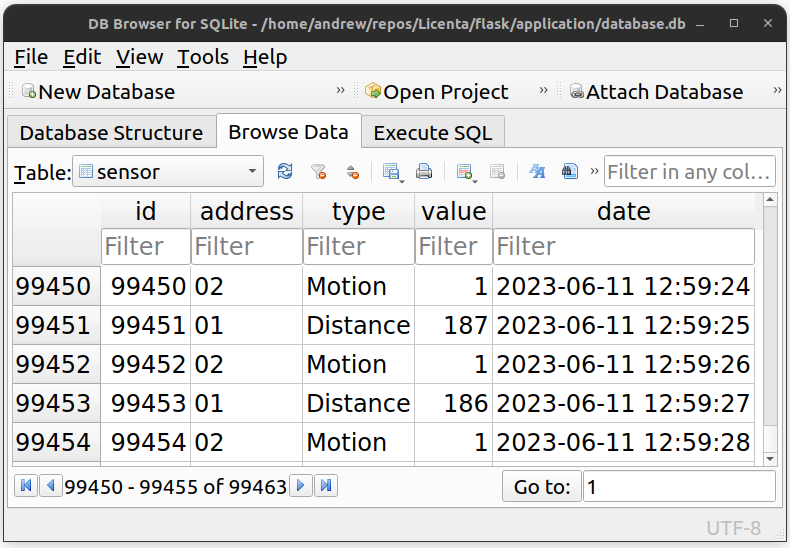
\includegraphics[width=0.7\textwidth]{14}
	\caption{Informațiile oferite de DB Browser for SQLite}
	\label{fig:14}
\end{figure}

Există două tabele în \textbf{/flask/application/models.py}: \textbf{Sensor} și \textbf{AdvancedSensor}, ambele stocând date (figura \ref{fig:14}) precum id-ul, numele, valoarea și data la care a fost adăugată înregistrarea senzorului în baza de date.

\break

Senzorii emit date odată la două secunde care trebuie stocate. Pentru acest lucru, am creat un fir de execuție nou care inserează fiecare citire pe care serverul o primește folosindu-se de codul din figura de mai jos.

\begin{lstlisting}[style=python, label=code:db]
EXPECTED_SIZE = struct.calcsize("<16sL")
def update_database(app, db):
	try:
		while True:
			network.update()
			while network.available():
				header, payload = network.read()
				sensor_type, value = struct.unpack("<16sL", payload[:EXPECTED_SIZE])
				sensor_type = sensor_type.decode('utf-8')
				sensor_type_clean = ''.join(letter for letter in sensor_type if letter.isalnum())
				address = header.to_string().split(' ')[3]
				
				with app.app_context()
					sensor_db_entry = Sensor(address=address, type=sensor_type_clean, value=value)
					db.session.add(sensor_db_entry)
					db.session.commit()
	except KeyboardInterrupt:
		print("powering down radio and exiting.")
		radio.power = False
\end{lstlisting}

În primă fază este calculată lungimea pachetelor transmise de senzori, aceștia conținând un cuvânt de 16 caractere și un număr întreg. Cât timp serverul este deschis, se vor citi aceste pachete, vor fi sanitizate și de-serializate, operații ce vor rezulta în obținerea valorilor trimise de la senzor.
La final va fi creat un obiect de tipul \emph{Sensor} care va fi introdus în baza de date locală.


\section{Senzori statici}

Acest tip de device-uri stă la baza metodei de coletare a informațiilor despre casa respectivă și cea de generare a unui raport cu toate valorile din baza de date în intervalul cerut.

Figura \ref{fig:static} ne prezintă cum a fost creat un senzor static: un Arduino Nano care este cablat la senzorul de detectare a mișcării și modulul de transmitere a datelor. 

\begin{figure}[h]
	\centering
	\begin{subfigure}{0.45\textwidth}
		\centering
		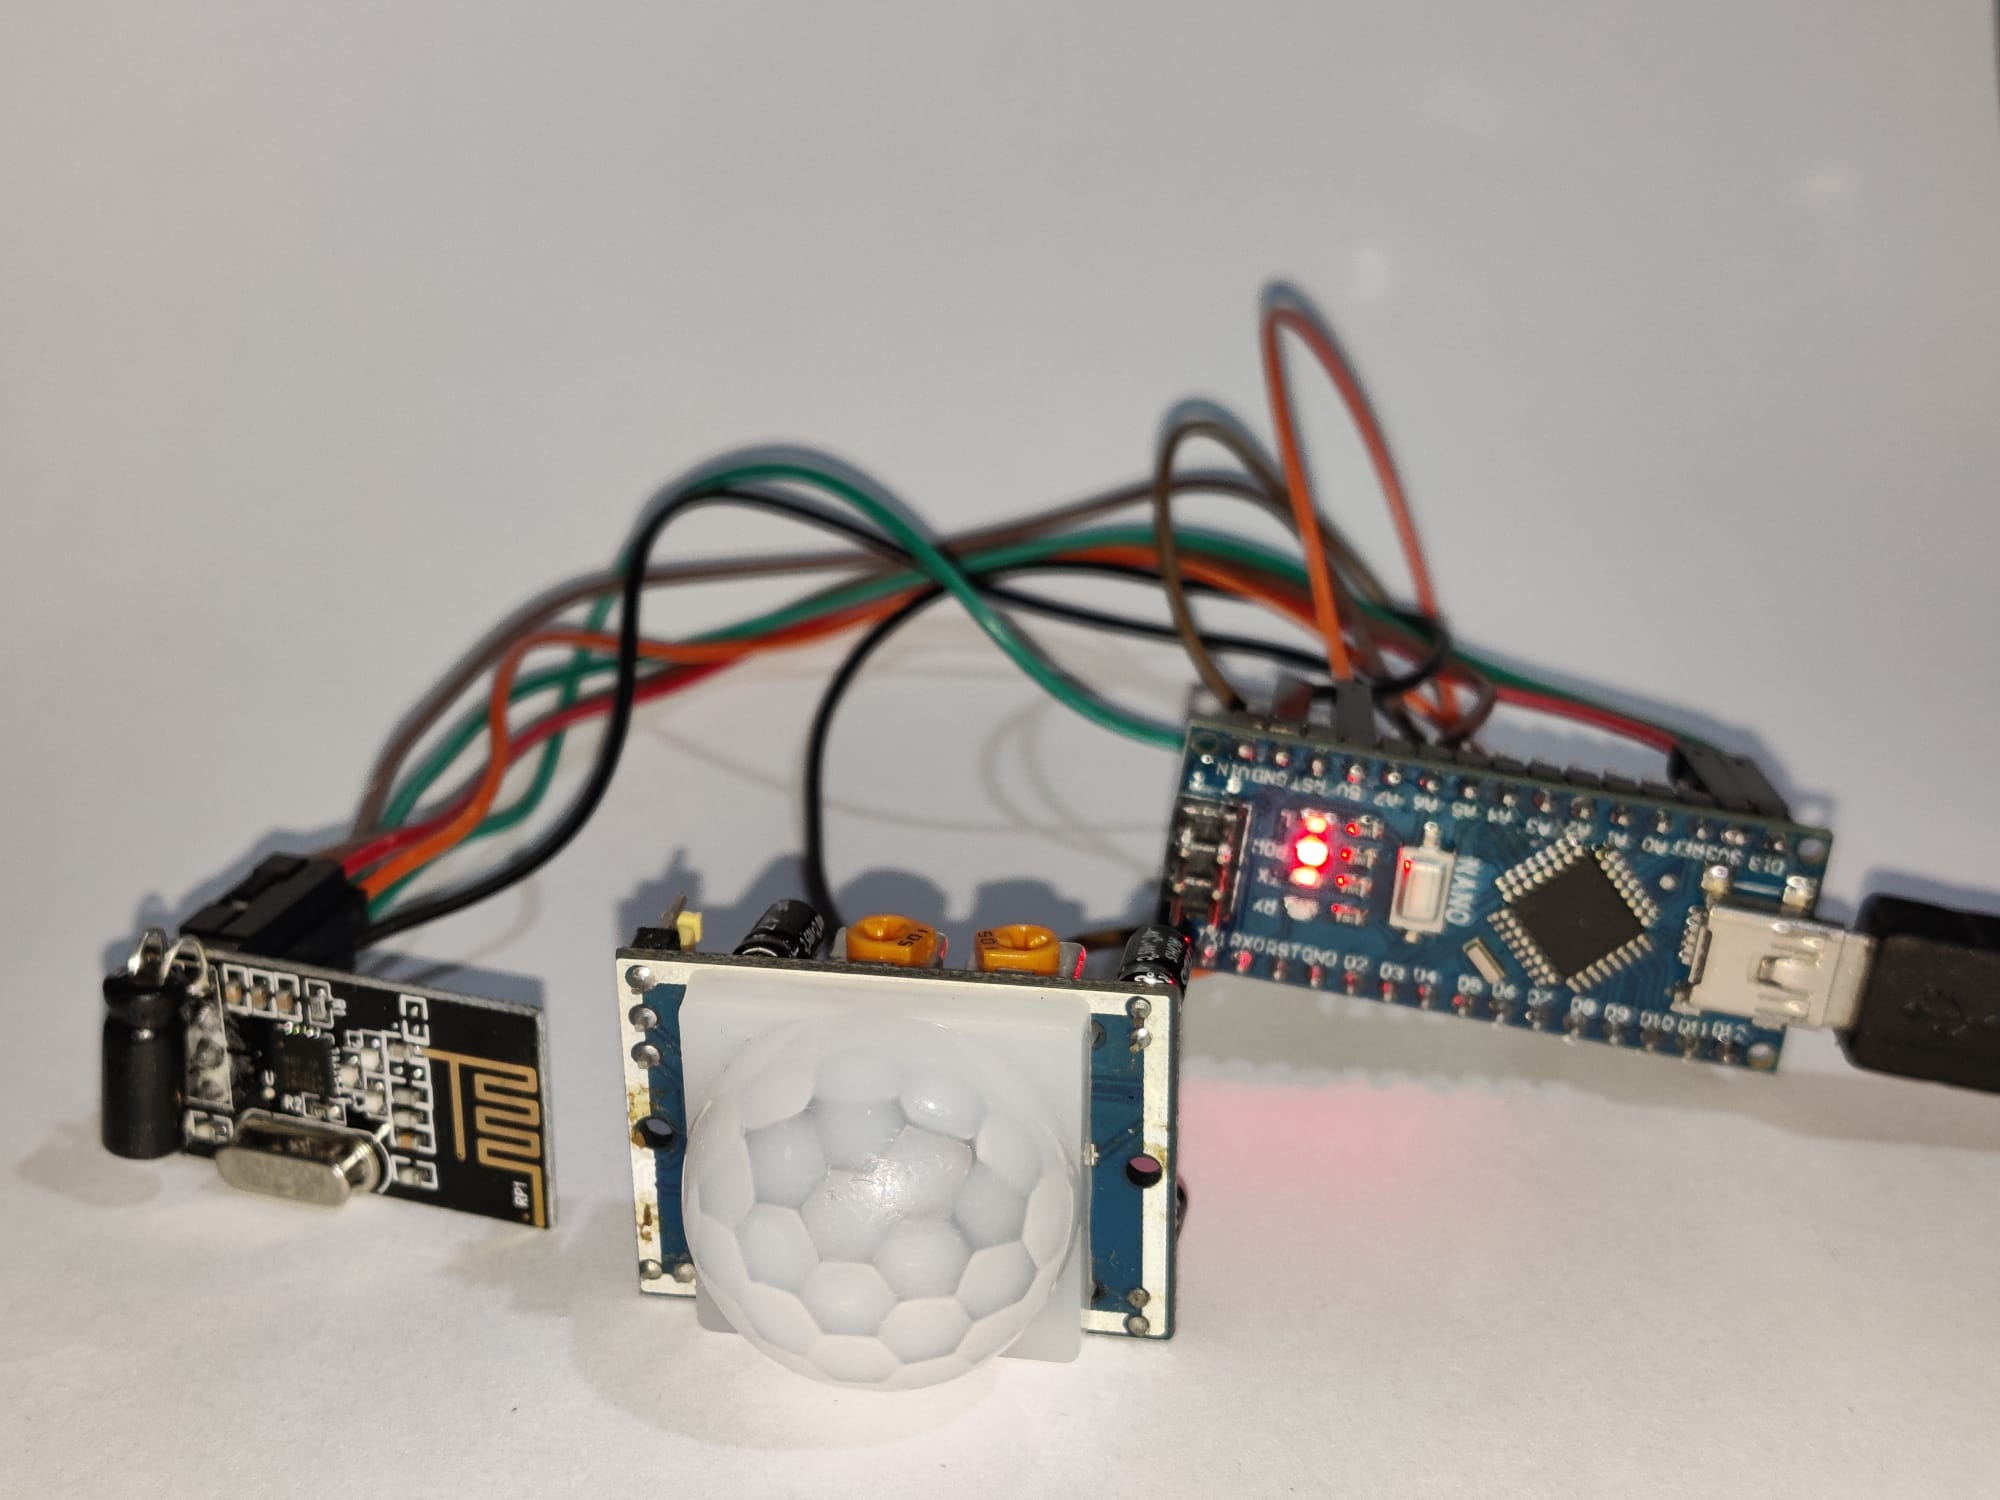
\includegraphics[width=\textwidth]{static}
		\caption{Arduino Nano cablat la senzorul de mișcare și modulul transmisie}
		\label{fig:static}
	\end{subfigure}
	\hfill
	\begin{subfigure}{0.45\textwidth}
		\centering
		
\includegraphics[width=\textwidth]{pir}
		\caption{Componenta piroelectrică}
		\label{fig:pir}
	\end{subfigure}
	\caption{Arduino și demonstrație}
	\label{fig:all2}
\end{figure}

Senzorul are 3 pini care trebuie conectați la placa de dezvoltare: împământarea, 5V și ieșirea. Ultimul pin emite un 0 logic dacă nu a detectat niciun obiect și 1 logic dacă a detectat o persoană sau un animal. Acest lucru este posibil datorită faptului că este emisă căldură în formă de radiații infra-roșii care alimentează componenta \emph{piroelectrică} (Figura \ref{fig:pir}) amplasată dedesubtul unei lentile Fresnel ce ajută focusarea acestor raze pe lentila senzorului. Modulul are încorporat două potențiometre: unul pentru reglarea razei de acțiune (până în 5 metri), iar celălalt pentru reglarea timpului de schimbare a valorii detectate (între 0.3 - 300 secunde). 

Odată alimentat la 5V, microcontroller-ul începe colectarea de date la un interval setat în faza configurării de către utilizator. În cazul meu, acesta este de două secunde. După ce acest interval a trecut, va fi creat un pachet ce conține ID-ul și tipul modulului, valoarea și data la care a fost făcută măsurătoarea. 

\section{Senzori dinamici}

Senzorii dinamici dețin o complexitate mai ridicată față de tipul anterior prezentat datorită faptului că pot trimite și primi date simultan de la server.

Imaginea \ref{fig:dinamic} demonstrează o utilitate simplă a modulului albastru care comută orice consumator ce poate fi alimentat de la priză. Fiecare componentă albastră acționează asemănător unui întrerupător care este controlat apăsând unul din butoanele prezente în interfața aplicației de telefon (Figura \ref{fig:8}). Ruta apelată este predefinită de către utilizator în faza de configurare a senzorului.

Pentru ca persoana ce deține soluția Smart Home să aibă cele mai recente funcționalități, senzorii își vor trimite toate informațiile serverului, acesta ulterior modificându-le în baza de date.

\begin{figure}[h]
	\centering
	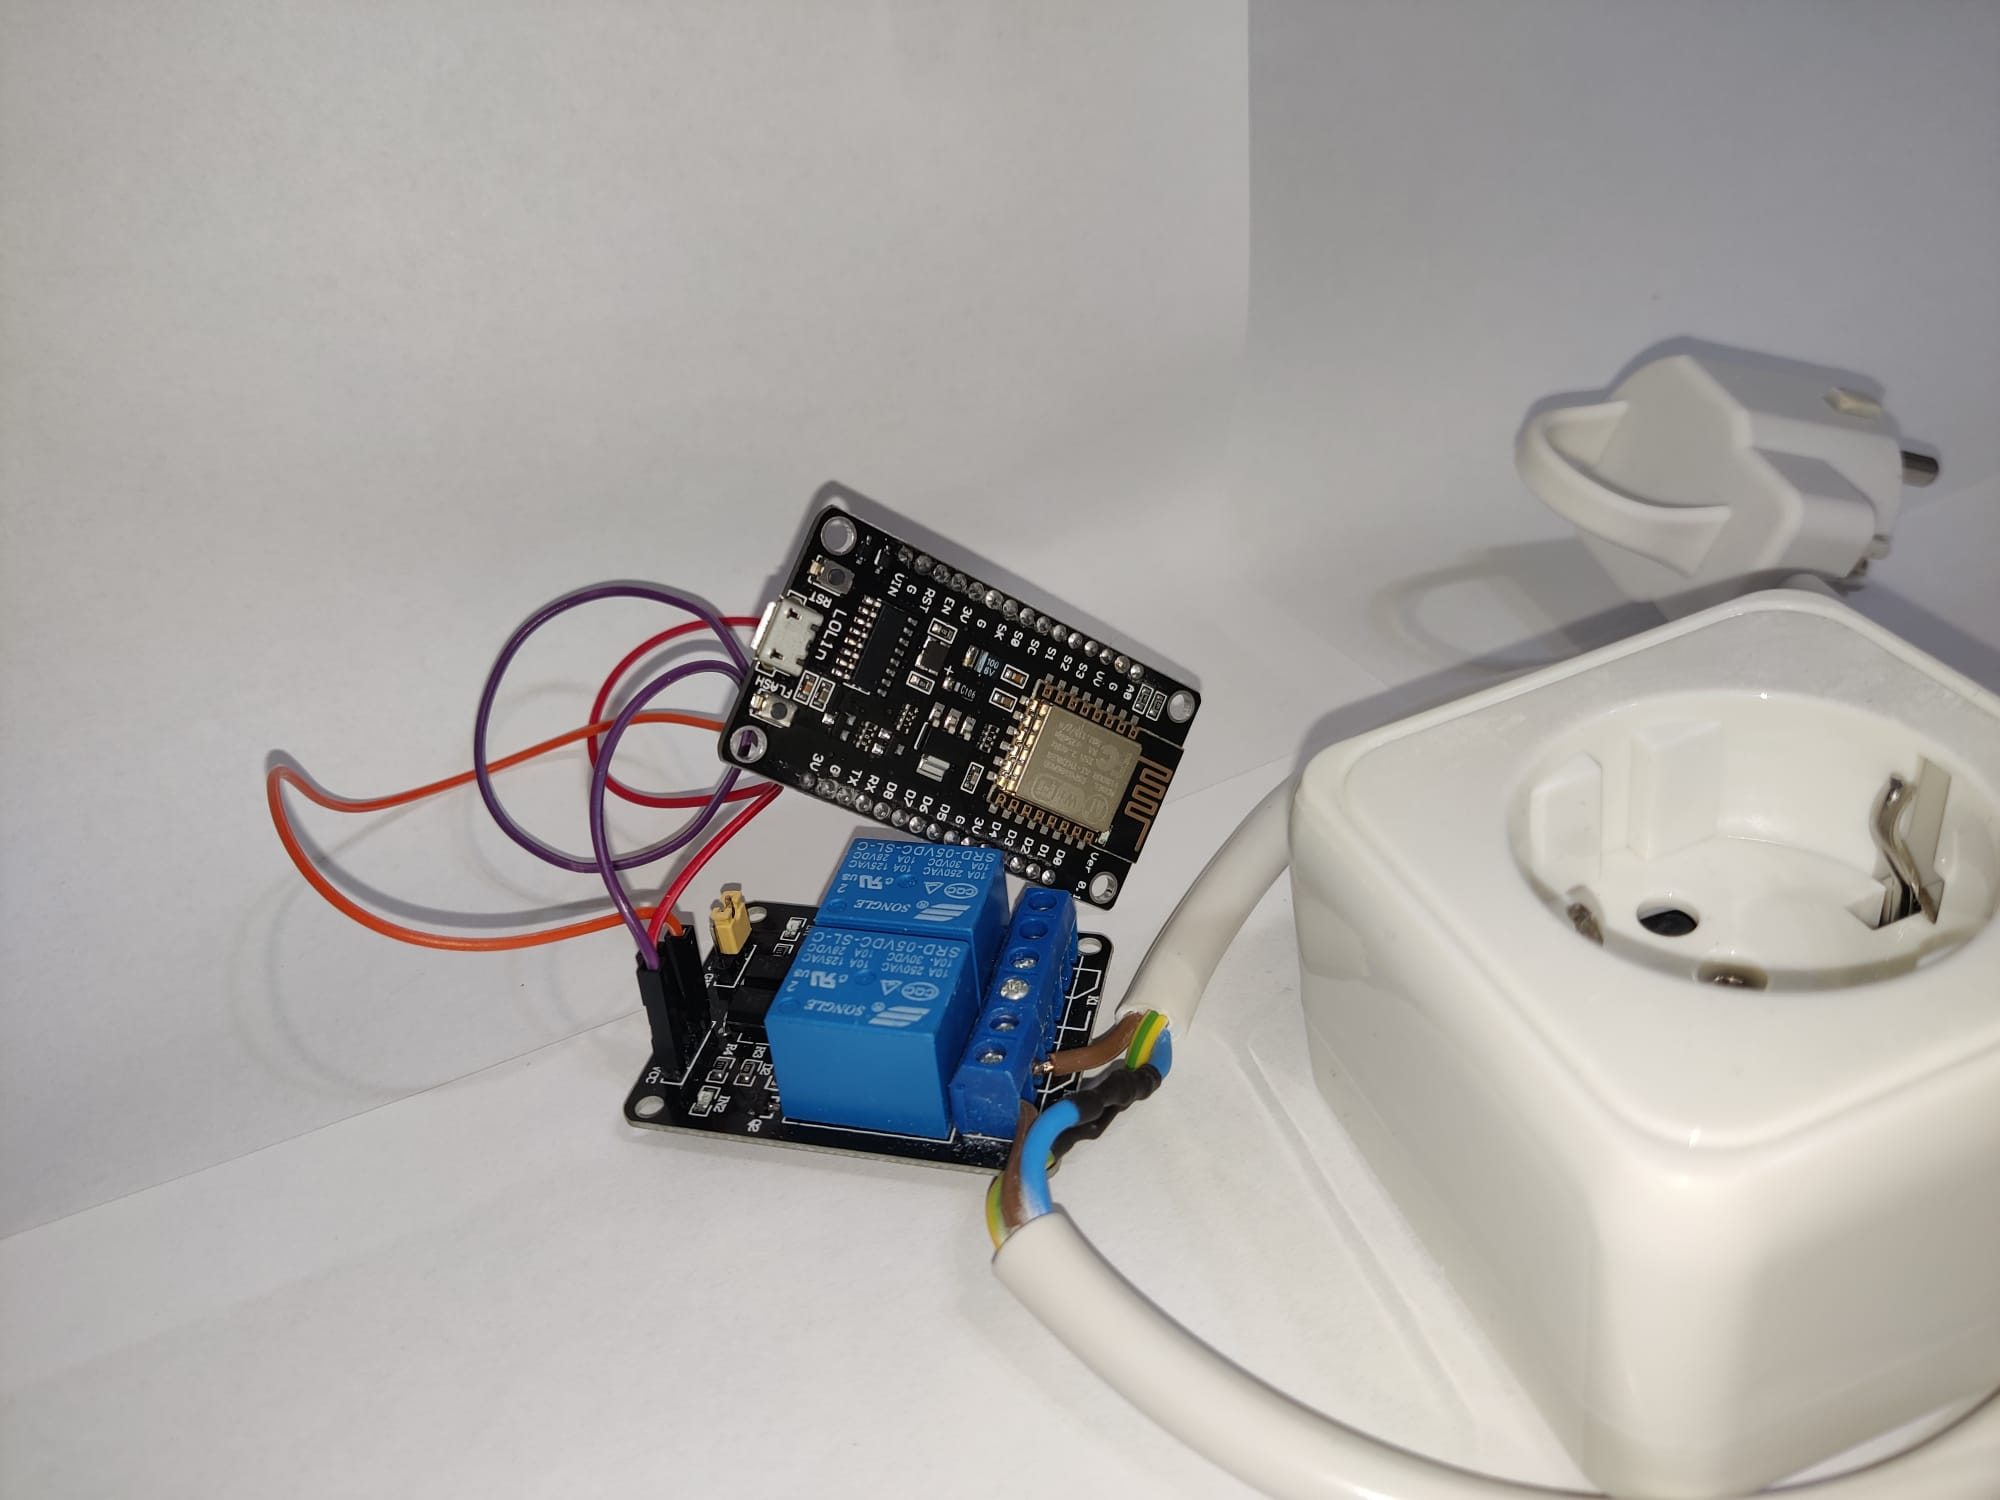
\includegraphics[width=0.6\textwidth]{dinamic}
	\caption{ESP8266 cu modul releu alimentat la 220V}
	\label{fig:dinamic}
\end{figure}

\section{Versionarea}

Câteva din caracteristicile licenței au solicitat folosirea metodologiei de \emph{branching}, schimbările codului fiind aplicate pe o copie a celui original. Am ales astfel să folosesc utilitarul \textbf{git}\footnote{\url{https://git-scm.com/}}, proiectul fiind postat pe \textbf{Github}\footnote{\url{https://github.com/}.} deoarece sunt familiar cu ambele tehnologii. Autentificarea bazată pe chei a fost folosită pentru a evita introducerea parolei contului la fiecare \emph{push} sau \textbf{pull}.

\newpage

\section{Fiabilitatea transmisiei datelor}

\begin{figure}[h]
	\centering
	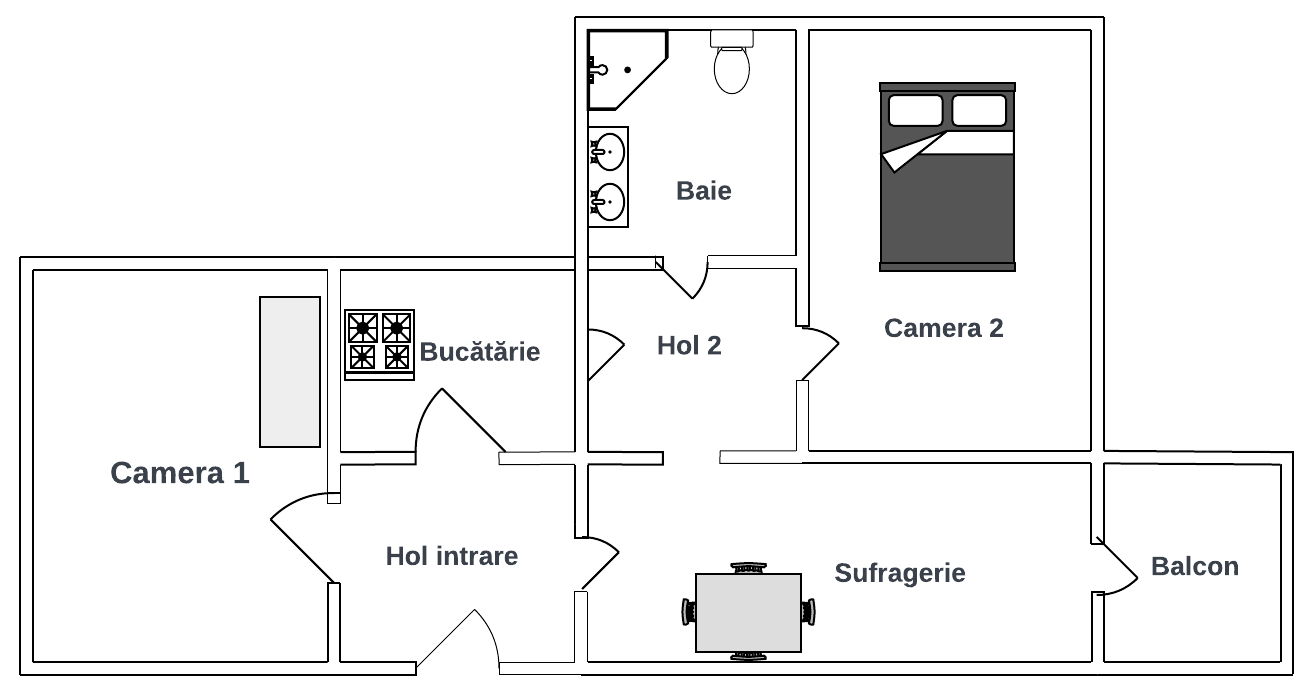
\includegraphics[width=1\textwidth]{apartament}
	\caption{Scema apartamentului unde au fost pozitionați senzorii}
	\label{fig:apartament}
\end{figure}

O conexiune stabilă este necesară pentru ca stația de bază (serverul) să primească pachetele de date de la toți senzorii. Distanța dintre cele două joacă un rol important în asigurarea trimiterii corecte a pachetelor.

Fiind folosită banda de 2.4GHz pentru comunicare, există multipli factori ce pot afecta transmisia informațiilor între module:
\begin{itemize}
	\item Puterea semnalului: aceasta scade pe măsură ce distanța dintre senzori și stația de bază crește.
	
	\item Obstacole: pereții și mobila diminuează semnificativ semnalul
	
	\item Interferența: alte dispozitive ce folosesc aceeași bandă de comunicare pot corupe pachetele trimise (cuptorul cu microunde, stații Wi-Fi)
\end{itemize}

Pentru a spori fiabilitate transmisiei, putem aplica următoarele  remedii: poziționarea stației de bază în centrul senzorilor, utilizarea extensiilor de semnal și deconectarea surselor de interferență.

Figura \ref{fig:apartament} reprezintă planul apartamentului în care este instalată soluția "Home Smartify". Pentru acest test, toți senzorii (distanță, mișcare și comutatorul) au fost amplasați în \emph{Camera 1}, iar stația de bază în \emph{Camera 2}. Din cauza pereților tuturor camerelor ce se află între dispozitive și stație, am obținut că senzorii statici (care nu au un mecanism de confirmare pentru primirea pachetelor) au avut \textbf{4} din cele 10 pachete emise cu succes, iar cei dinamici au avut 100\% rata de succes.

Testul a fost condus și cu stația de bază mai aproape de senzori (Camera 1), și anume în \emph{Sufragerie}. Fiindcă există o cale directă între aceste două încăperi, toți senzorii au avut o rată de transmisie de 100\%, chiar și cu ușile intermediare închise.

Bazându-ne pe rezultatele de mai sus, putem concluziona că proximitatea dintre senzori și stație afectează semnificativ rata de succes a transmisiei, fiind necesară o distanță optimă între toți senzorii și server.